\chapter{Results}

	\section{Opinions on educational and fun games}
		\begin{figure}[] 
		\centering 
		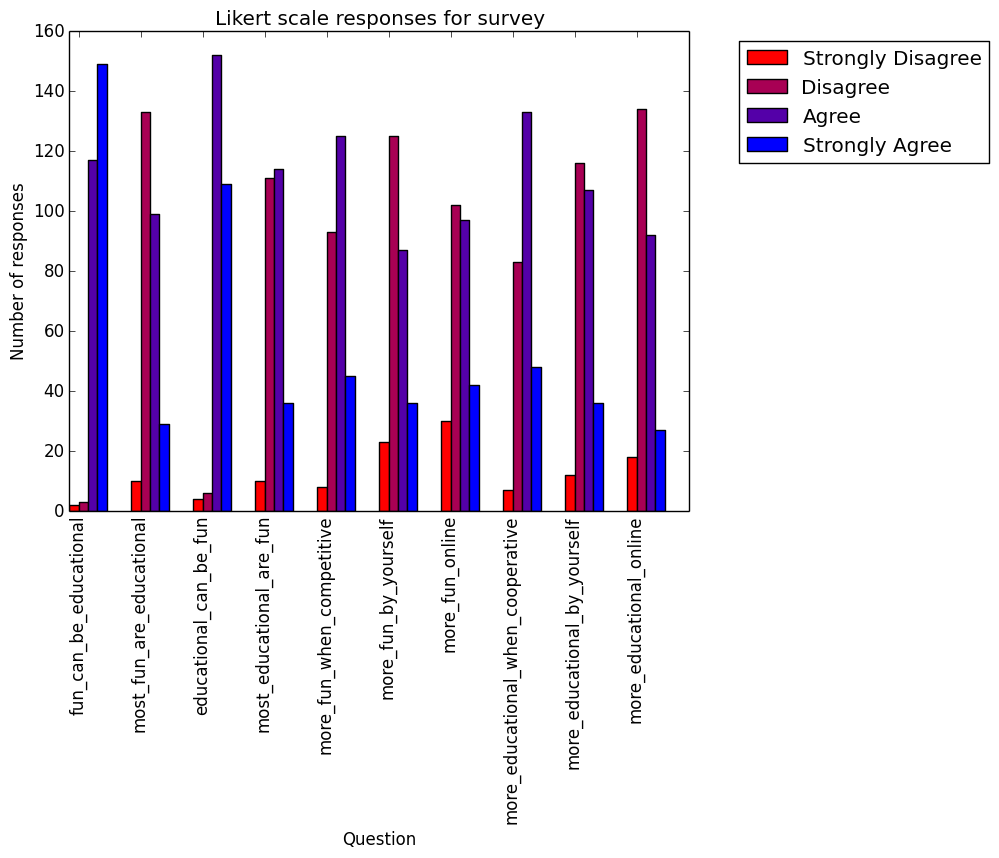
\includegraphics[width=\textwidth]{survey_likert.png} 
		\caption{Likert scale responses for several questions on fun and educational games.}
		\end{figure}
	These are the aggregated responses to the opinion Likert scale questions introduced in the very first part of the survey. While they don't have any influence on our results or analysis, it's interesting to note what kind of opinions or mindset workers when they begin taking the survey.

	These questions include opinions about whether educational games can be fun (or vice versa), and if most of them are. There were also some questions about fun/educational games being competitive/cooperative, and more fun/educational if playing online/offline, solo or with friends.

	The most interesting sections of this chart are the ``Fun/educational games can be educational/fun'' sections; almost unanimous agreement there. However, ``most fun games are educational'' met with a substantial amount of disagreement. This is expected; games that are commonly considered fun include shooters, adventure and action games. In addition, the ``most educational games are fun'' section was far more evenly distributed, implying that a substantial amount of people think educational games aren't fun.

	\clearpage

	\section{Quiz Results}
		This section contains results of all of the quiz responses, displayed in 3 graphs. The pre-quiz and post-quiz graphs indicate how many responses were received with a specific grade, from 0\% to 100\%. The score differences graphs indicate how many responses improved from the pre-quiz to the post-quiz, and by how much.

		For each graph, I'll include some non-statistical observations and insights. For detailed statistical analysis, see the Analysis chapter.

		\subsection{Aggregate Quiz Scores}

			\begin{figure}[] 
			\centering 
			\begin{minipage}[b]{0.45\linewidth}
			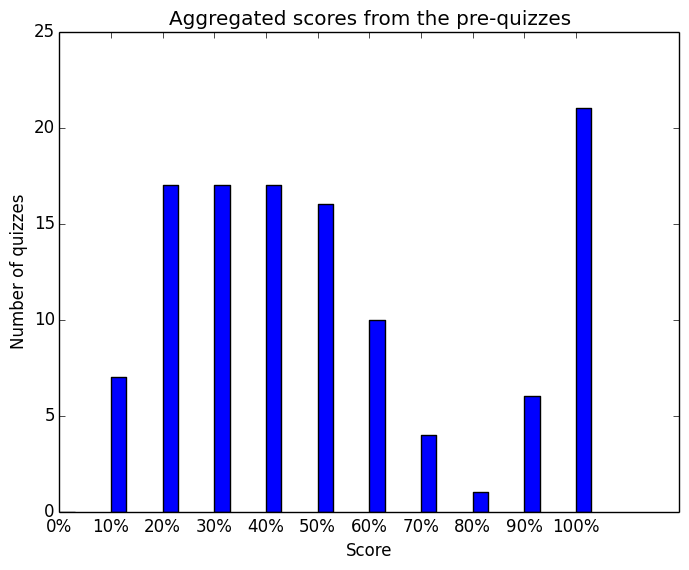
\includegraphics[width=\textwidth]{general_pre.png} 
			\caption{The aggregate pre-quiz scores across all games.}
			\end{minipage}
			\quad
			\begin{minipage}[b]{0.45\linewidth}
			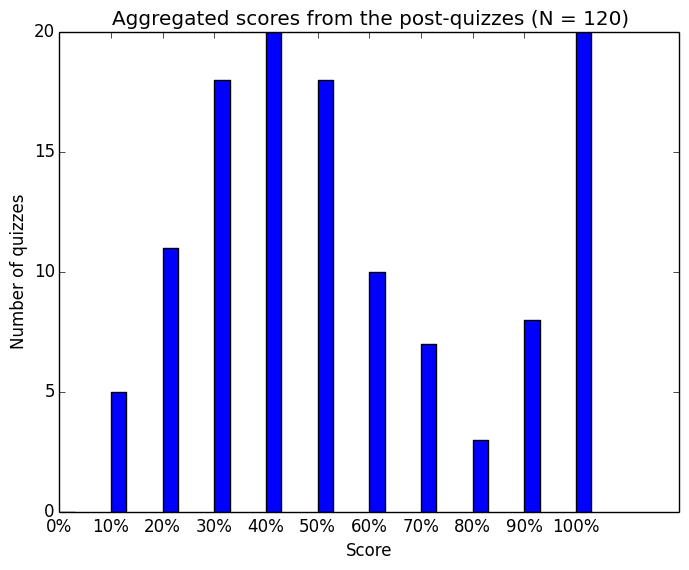
\includegraphics[width=\textwidth]{general_post.png} 
			\caption{The aggregate post-quiz scores across all games.}
			\end{minipage}
			\end{figure}

			\begin{figure}[] 
			\centering 
			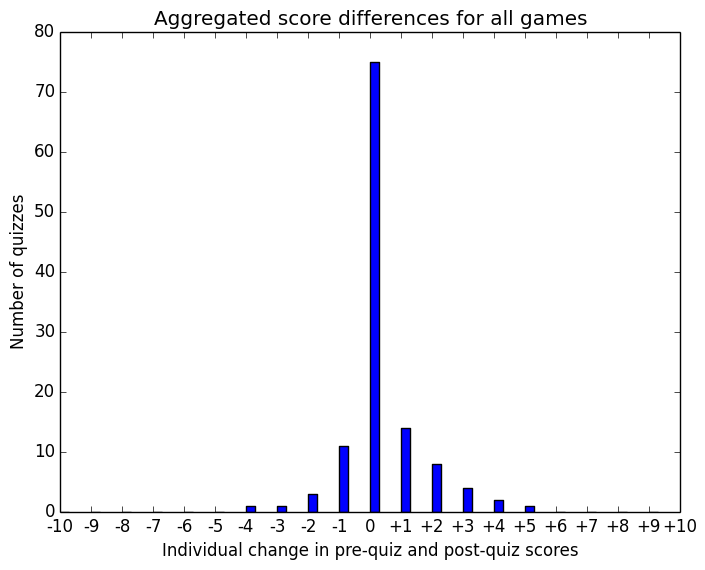
\includegraphics[width=\textwidth]{general_results.png} 
			\caption{The aggregate score differences across all games.}
			\end{figure}



			The complete lack of a bell curve on our pre-quiz (Figure 6.2) and post-quiz (Figure 6.3) aggregates means that our quizzes may not be as evenly distributed as we'd like. As explained in the next chapter, aggregating the responses across all of our quizzes does not yield score increases that are statistically significantly different from zero. 

			The massive peak in the score differences chart (Figure 6.4) shows how little of a change there was in the majority of the responses. This means that most quizzes had zero improvement or change in score. This was unexpected, because the pre-quiz and post-quiz for each worker was almost identical; with very little variation in the answers.

			\clearpage

		\subsection{Darfur Quiz Scores}

			\begin{figure}[] 
			\centering 
			\begin{minipage}[b]{0.45\linewidth}
			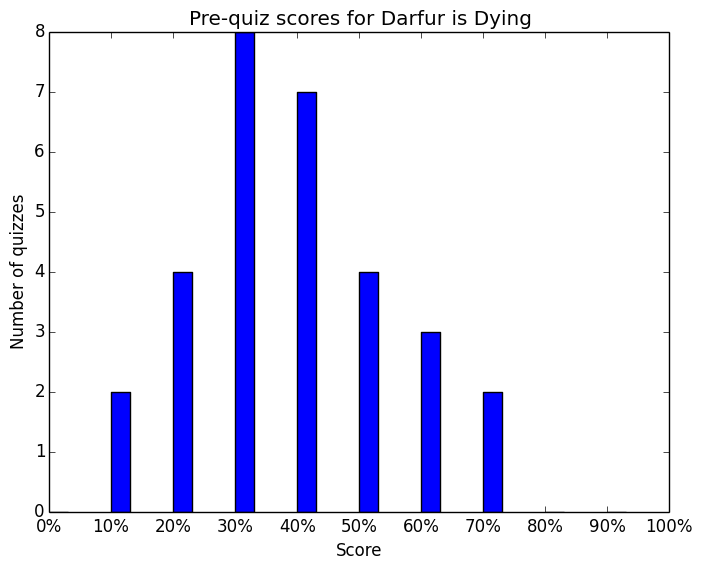
\includegraphics[width=\textwidth]{darfur_pre.png} 
			\caption{The pre-quiz scores for Darfur is Dying.}
			\end{minipage}
			\quad
			\begin{minipage}[b]{0.45\linewidth}
			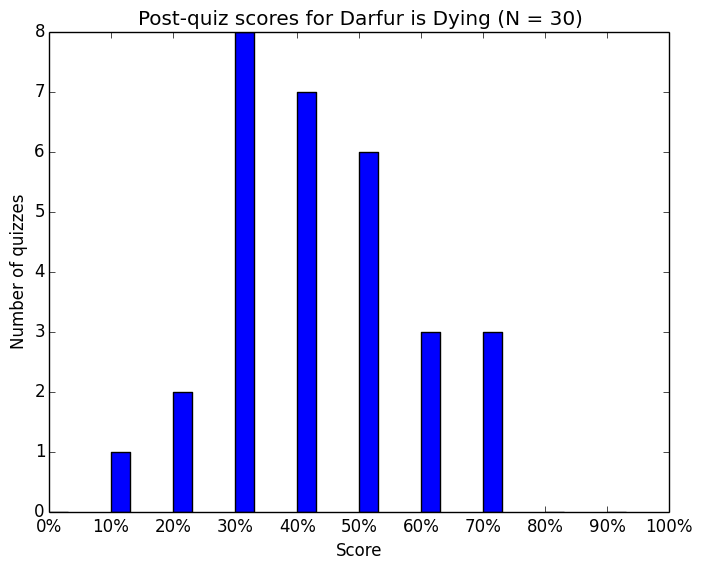
\includegraphics[width=\textwidth]{darfur_post.png} 
			\caption{The post-quiz scores for Darfur is Dying.}
			\end{minipage}
			\end{figure}

			\begin{figure}[] 
			\centering 
			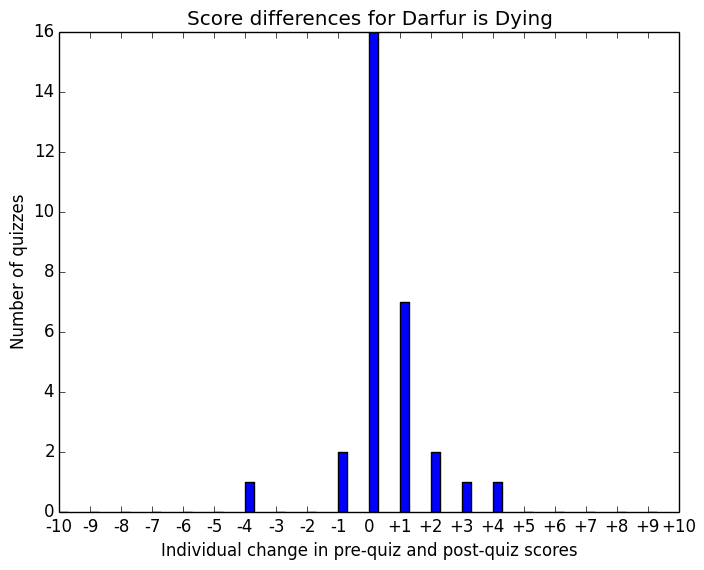
\includegraphics[width=\textwidth]{darfur_results.png} 
			\caption{The score differences for Darfur is Dying.}
			\end{figure}

			The pre-quiz (Figure 6.5) and post-quiz (Figure 6.6) graphs show a roughly standard distribution. The score differences graph (Figure 6.7) shows the massive peak around zero, with minor improvements.

			\clearpage

		\subsection{The Oregon Trail Quiz Scores}		

			\begin{figure}[] 
			\centering 
			\begin{minipage}[b]{0.45\linewidth}
			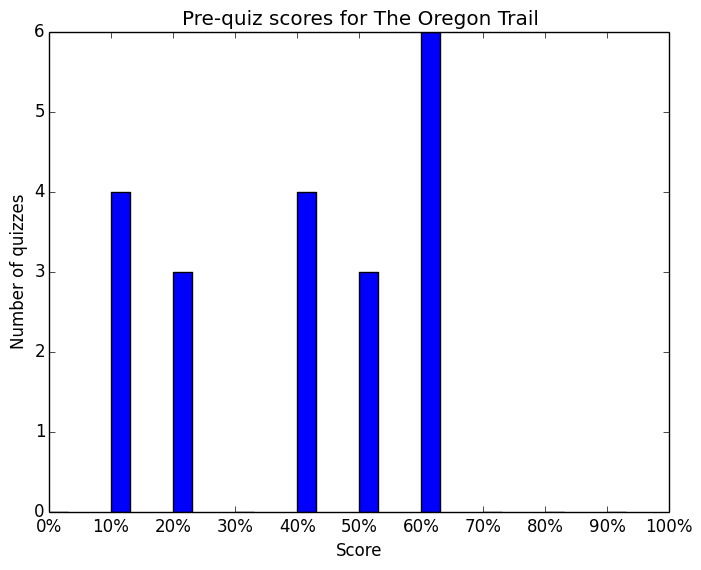
\includegraphics[width=\textwidth]{oregon_pre.png} 
			\caption{The pre-quiz scores for The Oregon Trail.}
			\end{minipage}
			\quad
			\begin{minipage}[b]{0.45\linewidth}
			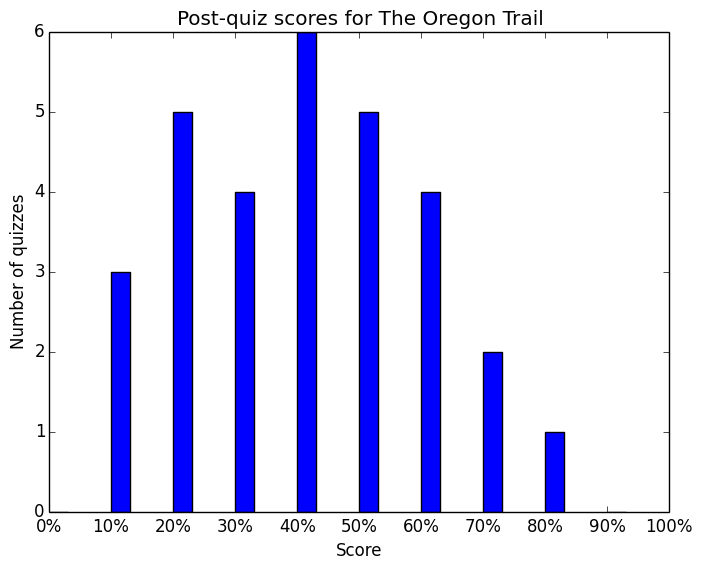
\includegraphics[width=\textwidth]{oregon_post.png} 
			\caption{The post-quiz scores for The Oregon Trail.}
			\end{minipage}
			\end{figure}
			
			\begin{figure}[] 
			\centering 
			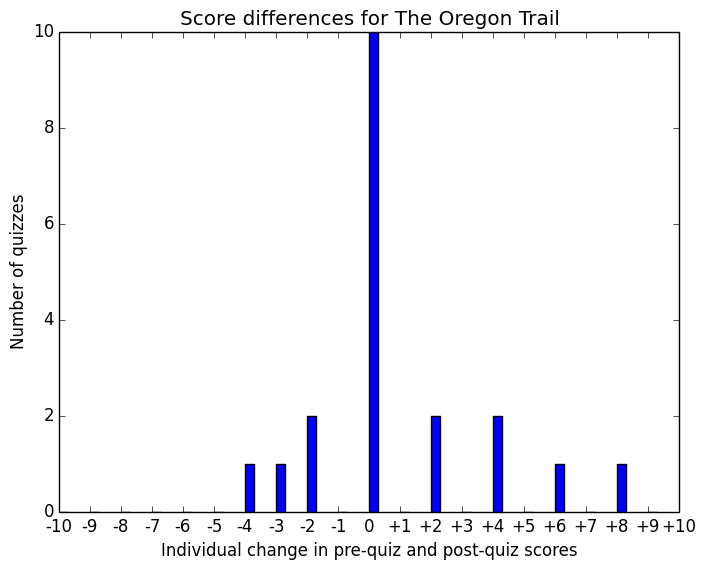
\includegraphics[width=\textwidth]{oregon_results.png} 
			\caption{The score differences for The Oregon Trail.}
			\end{figure}

			The pre-quiz (Figure 6.8) and post-quiz (Figure 6.9) graphs show an increase in some scores, although there was almost no change for the majority of the quizzes (Figure 6.10)

			\clearpage

		\subsection{Number Munchers Quiz Scores}

			\begin{figure}[] 
			\centering 
			\begin{minipage}[b]{0.45\linewidth}
			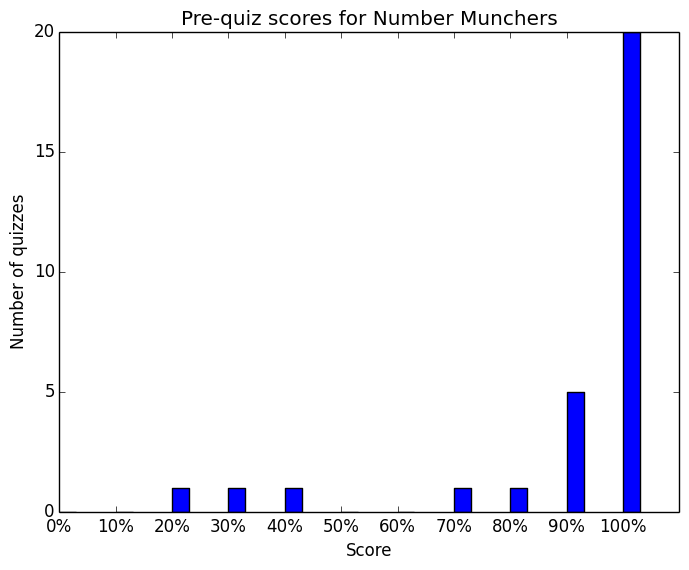
\includegraphics[width=\textwidth]{munchers_pre.png} 
			\caption{The pre-quiz scores for Number Munchers.}
			\end{minipage}
			\quad
			\begin{minipage}[b]{0.45\linewidth}
			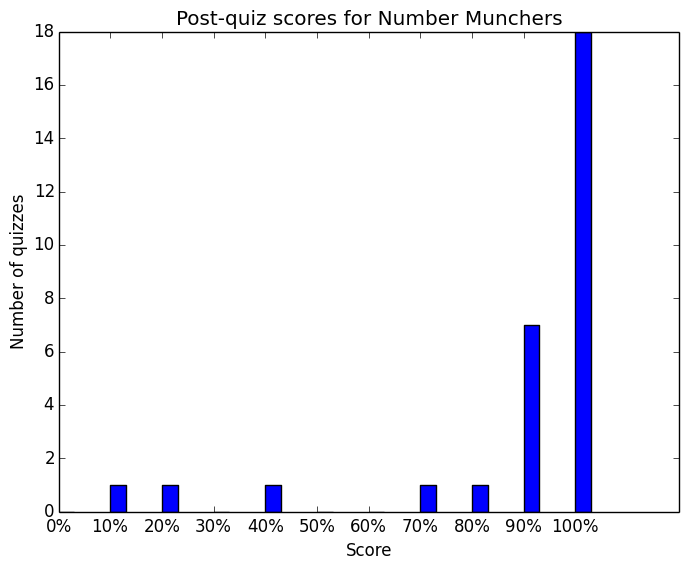
\includegraphics[width=\textwidth]{munchers_post.png} 
			\caption{The post-quiz scores for Number Munchers.}
			\end{minipage}
			\end{figure}

			\begin{figure}[] 
			\centering 
			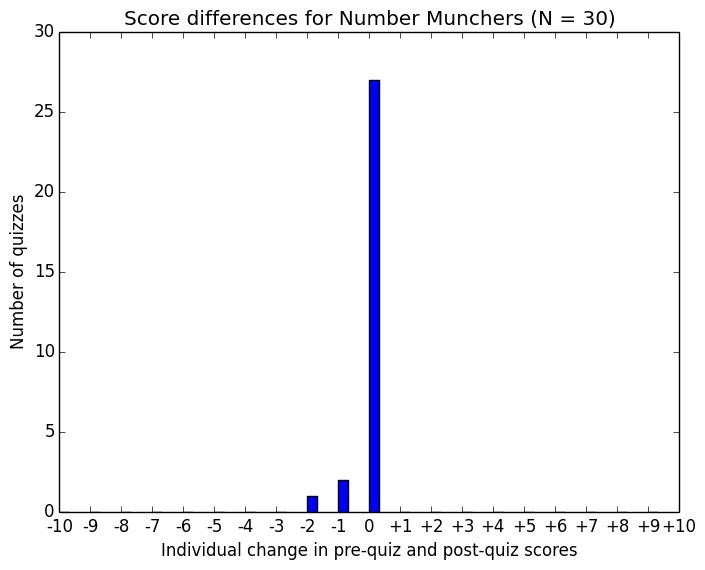
\includegraphics[width=\textwidth]{munchers_results.png} 
			\caption{The score differences for Number Munchers.}
			\end{figure}

			The pre-quiz (Figure 6.11) and post-quiz (Figure 6.12) obviously ended up skewed towards 100\%. This is likely caused by the simplicity of the quiz; simple arithmetic is easy for Mechanical Turk workers aged 18+ to do, and some are likely assisted by a calculator (even though we expressly asked them not to use one).

			The score differences graph (Figure 6.13) actually shows zero positive improvements to quiz scores, with only 3 or 4 being negative.

			This is a clear example of the ceiling effect. Because the workers scored so highly on the pre-quiz and post-quiz, we can assume that the quiz was not difficult enough. If the quiz were more difficult, we would see more workers getting lower scores. This would result in a better distribution of scores, and more useful information in score differences.

			\clearpage

		\subsection{Light Bot Quiz Scores}

			\begin{figure}[] 
			\centering 
			\begin{minipage}[b]{0.45\linewidth}
			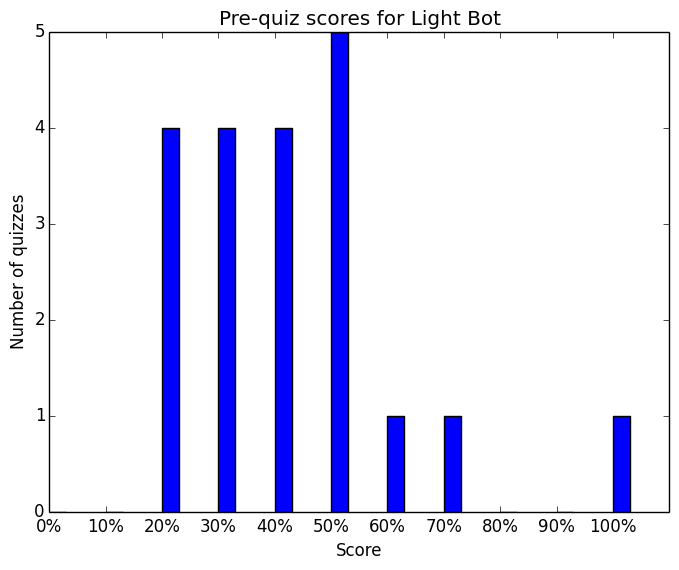
\includegraphics[width=\textwidth]{lightbot_pre.png} 
			\caption{The pre-quiz scores for Light Bot.}
			\end{minipage}
			\quad
			\begin{minipage}[b]{0.45\linewidth}
			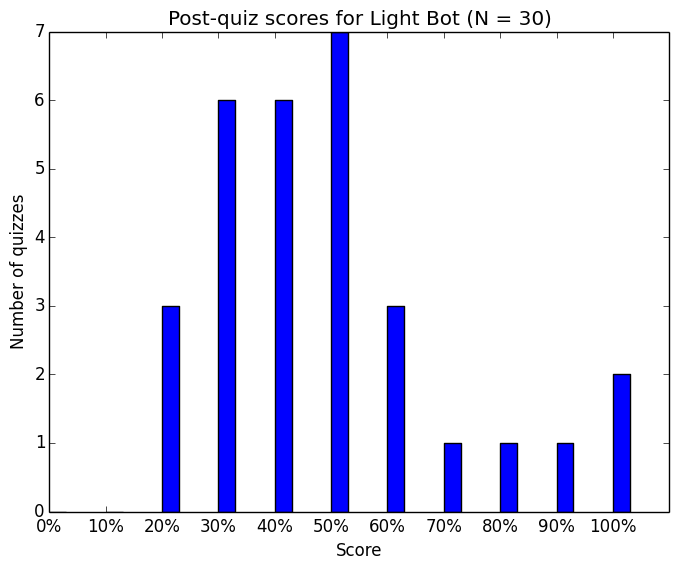
\includegraphics[width=\textwidth]{lightbot_post.png} 
			\caption{The post-quiz scores for Light Bot.}
			\end{minipage}
			\end{figure}

			\begin{figure}[] 
			\centering 
			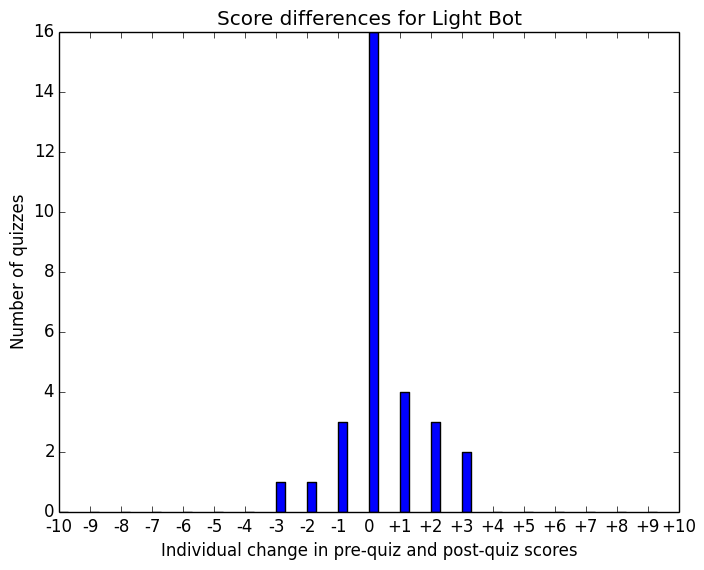
\includegraphics[width=\textwidth]{lightbot_results.png} 
			\caption{The score differences for Light Bot.}
			\end{figure}

			\textit{Light Bot's} pre-quiz (Figure 6.14) and post-quiz (Figure 6.15) scores show a roughly standard distribution skewed toward the high end. This could mean that some reviewers were already familiar with this material, or that they were so engaged with the questions that they spent extra time on them. In either case, the ceiling effect will slightly affect our score differences results (Figure 6.16). The score differences show a roughly standard disribution with a large peak at 0.

			\clearpage

		\section{Rubric Scores}
			This section contains the scoring results for each rubric item. For each rubric item, a bar graph is given for each game. These graphs are shown in Figures 6.17 through 6.29. The bar graph contains the scores that the game recieved for that rubric item.

			An alternate visualization of this data, where each game has a bar graph for all of the rubric items, can be found in the next section.


			\subsection{Adaptive Difficulty}
				\begin{figure}[] 
				\centering 
				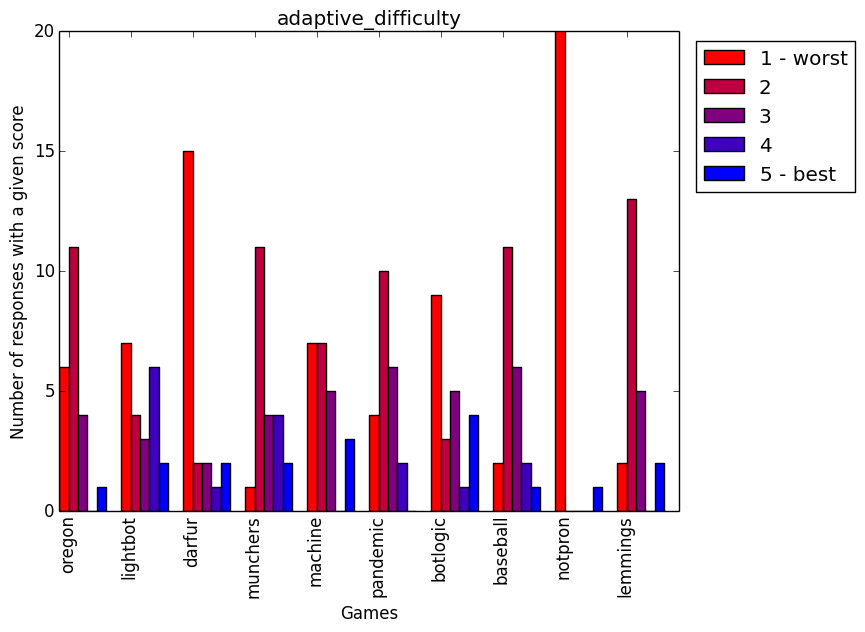
\includegraphics[width=\textwidth, height=.4\textheight, keepaspectratio=true]{adaptive_difficulty_scores.png} 
				\caption{Adaptive Difficulty}
				\end{figure}

				The most striking part of this graph is the obvious lack of adaptive difficulty present in \textit{Notpron}, and to some degree, \textit{Darfur is Dying}. This seems straightforward, as both \textit{Notpron} and \textit{Darfur is Dying} have no option to set difficulty. There are no games with large positive degrees of adaptive difficulty.

			\subsection{Checkpoint Frequency}
				\begin{figure}[] 
				\centering 
				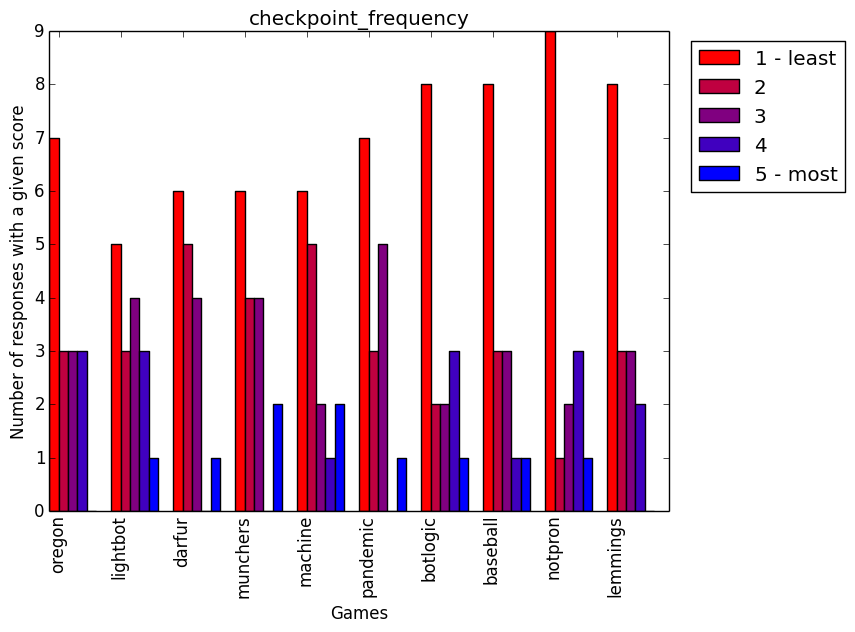
\includegraphics[width=\textwidth, height=.4\textheight, keepaspectratio=true]{checkpoint_frequency_scores.png} 
				\caption{Checkpoint Frequency}
				\end{figure}

				For checkpoint frequency, response was universally negative. This is concerning, because I was confident that some games (\textit{Notpron, The Incredible Machine, Light Bot}) had frequent checkpoints. This may imply that the prompt or selections were misleading.

			\subsection{Contextual Tutorials}
				\begin{figure}[] 
				\centering 
				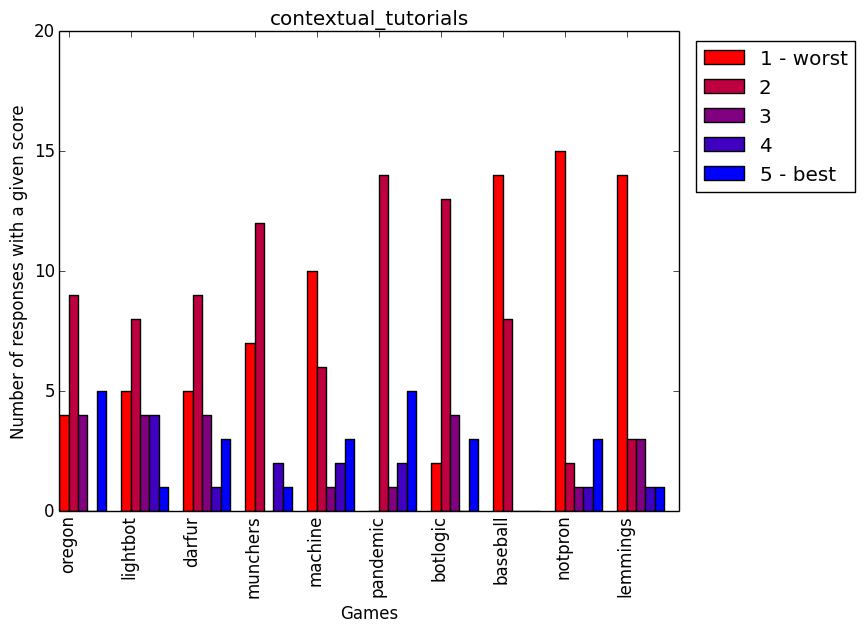
\includegraphics[width=\textwidth, height=.4\textheight, keepaspectratio=true]{contextual_tutorials_scores.png} 
				\caption{Contextual Tutorials}
				\end{figure}

				Response for contextual tutorials within the game was universally negative, with the most notable instance being \textit{Math Baseball}. This is expected; Math Baseball is a simple arithmetic game that provides no tutorials at all.

			\subsection{Encyclopedia Content}
				\begin{figure}[] 
				\centering 
				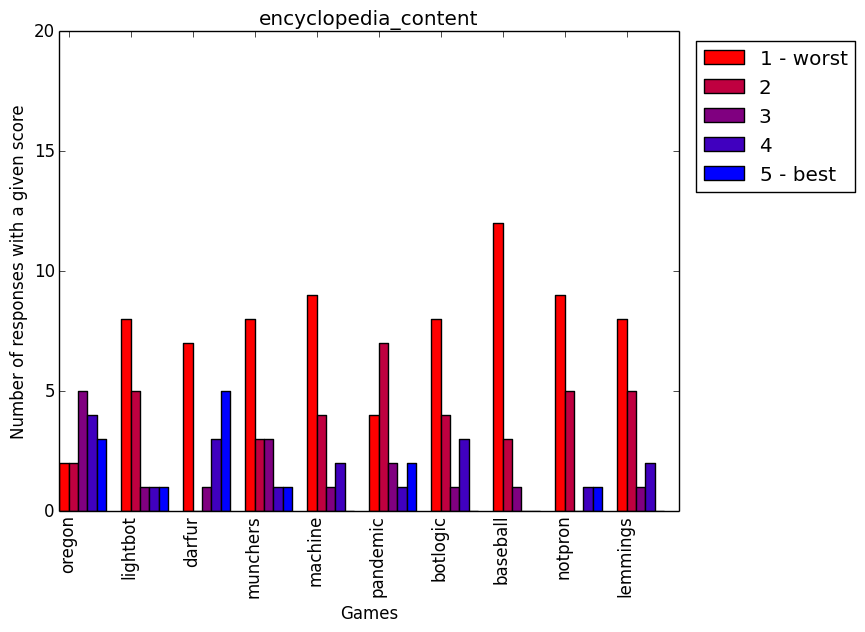
\includegraphics[width=\textwidth, height=.4\textheight, keepaspectratio=true]{encyclopedia_content_scores.png} 
				\caption{Encyclopedia Content}
				\end{figure}

				For the content of the game's encyclopedia, both \textit{The Oregon Trail} and \textit{Darfur is Dying} scored relatively highly. It's expected that both of these games (focused around historical/current events) seem to directly benefit from tangential learning.

			\subsection{Encyclopedia Location}
				\begin{figure}[] 
				\centering 
				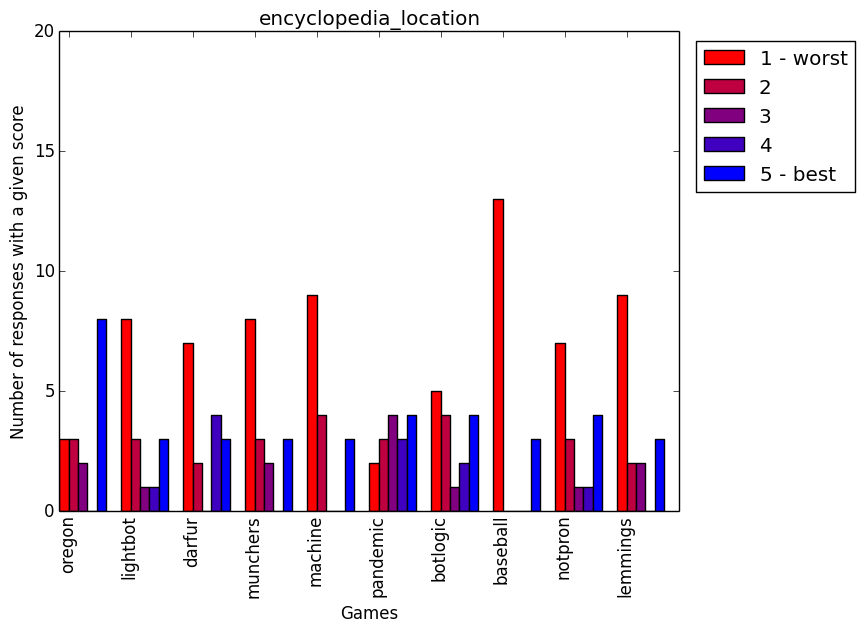
\includegraphics[width=\textwidth, height=.4\textheight, keepaspectratio=true]{encyclopedia_location_scores.png} 
				\caption{Encyclopedia Location}
				\end{figure}

				The only game that scored moderately well on the location of the game encyclopedia was \textit{The Oregon Trail}. This is expected; the introduction sequence of the game provides a lot of useful and historical information.

			\subsection{Freedom of exploration}
				\begin{figure}[] 
				\centering 
				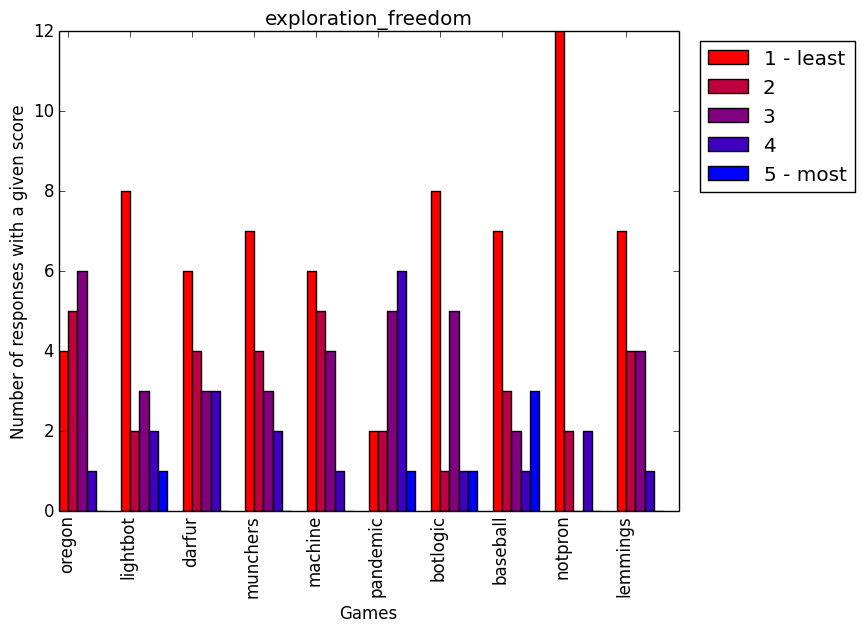
\includegraphics[width=\textwidth, height=.4\textheight, keepaspectratio=true]{exploration_freedom_scores.png} 
				\caption{Freedom of exploration}
				\end{figure}

				The only game that scored relatively well on freedom of exploration was \textit{Pandemic 2}. Players likely considered the `open world' format of the game as part of this rubric item.

			\subsection{Iterative Feedback}
				\begin{figure}[] 
				\centering 
				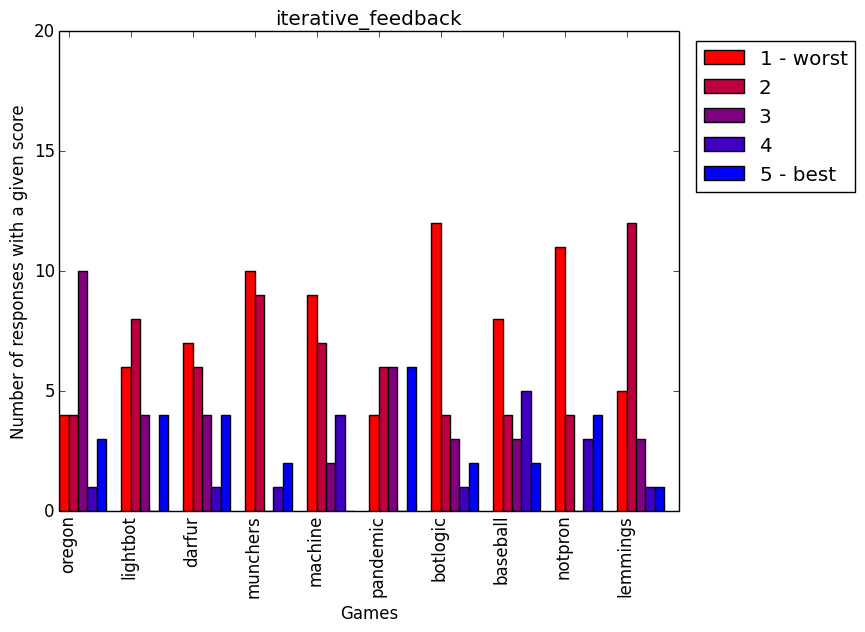
\includegraphics[width=\textwidth, height=.4\textheight, keepaspectratio=true]{iterative_feedback_scores.png} 
				\caption{Iterative feedback}
				\end{figure}

				Scores for games on iterative feedback were mixed at best. For \textit{The Oregon Trail}, players may have considered their frequent check-ins while along the trail useful, where they could ask for advice and make decisions.

			\subsection{Unorthodox problem-solving}
				\begin{figure}[] 
				\centering 
				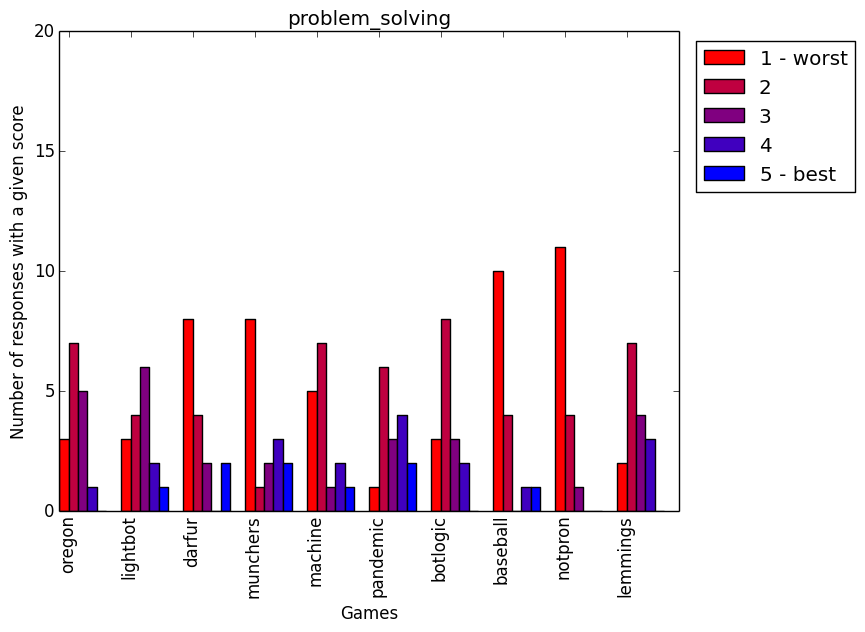
\includegraphics[width=\textwidth, height=.4\textheight, keepaspectratio=true]{problem_solving_scores.png} 
				\caption{Unorthodox problem-solving}
				\end{figure}

				Scores for unorthodox problem-solving were mixed; no significant exceptions to note.

			\subsection{Amount of referential material}
				\begin{figure}[] 
				\centering 
				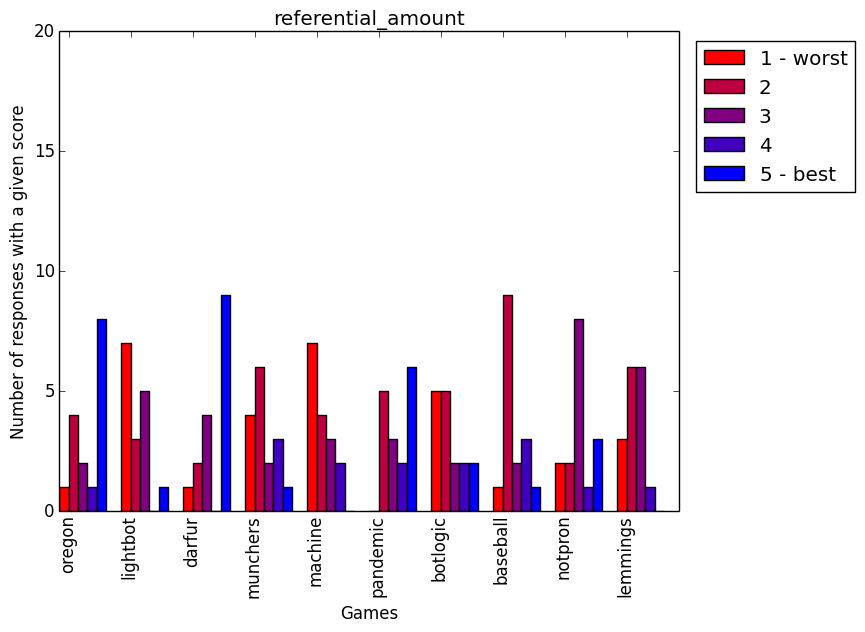
\includegraphics[width=\textwidth, height=.4\textheight, keepaspectratio=true]{referential_amount_scores.png} 
				\caption{Amount of referential material}
				\end{figure}

				Several games scored well on the amount of referential material in them. \textit{The Oregon Trail} and \textit{Darfur is Dying} were both expected, as well as \textit{Pandemic} to a degree. \textit{Notpron} was expected to do well, given the knowledge (web technology) that players are expected to know to be able to complete the game. However, \textit{Notpron} only scored in the middle of the range.

			\subsection{Popularity of referential material}
				\begin{figure}[] 
				\centering 
				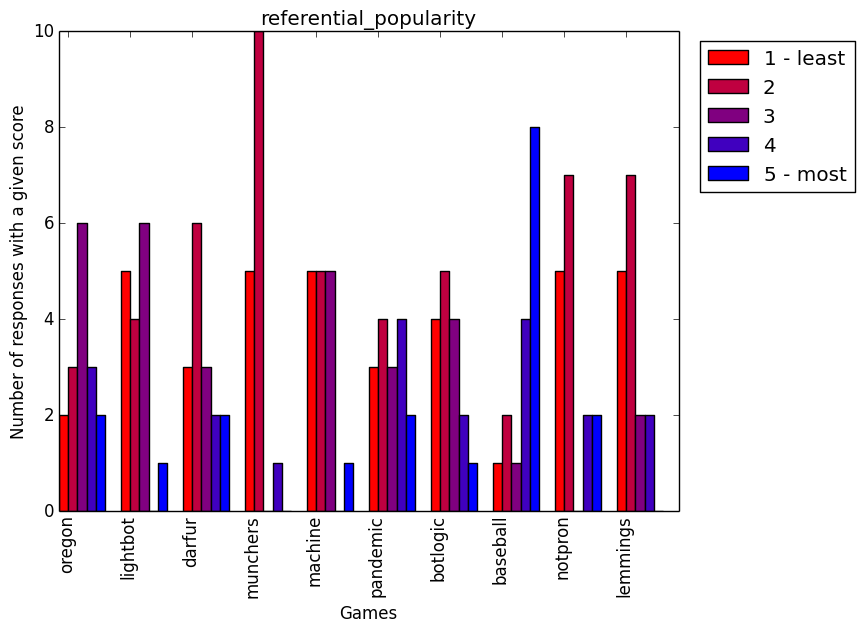
\includegraphics[width=\textwidth, height=.4\textheight, keepaspectratio=true]{referential_popularity_scores.png} 
				\caption{Popularity of referential material}
				\end{figure}

				\textit{Math Baseball's} popular referential material is considered basic arithmetic, something that is ubiquitous outside the game. It scored very highly. However, \textit{Number Munchers}, which covers extremely similar material, scored very poorly on this rubric item. This leads us to think that the rubric may be inconsistent, or additional research may need to be done.

			\subsection{Rewards for knowing referential material}
				\begin{figure}[] 
				\centering 
				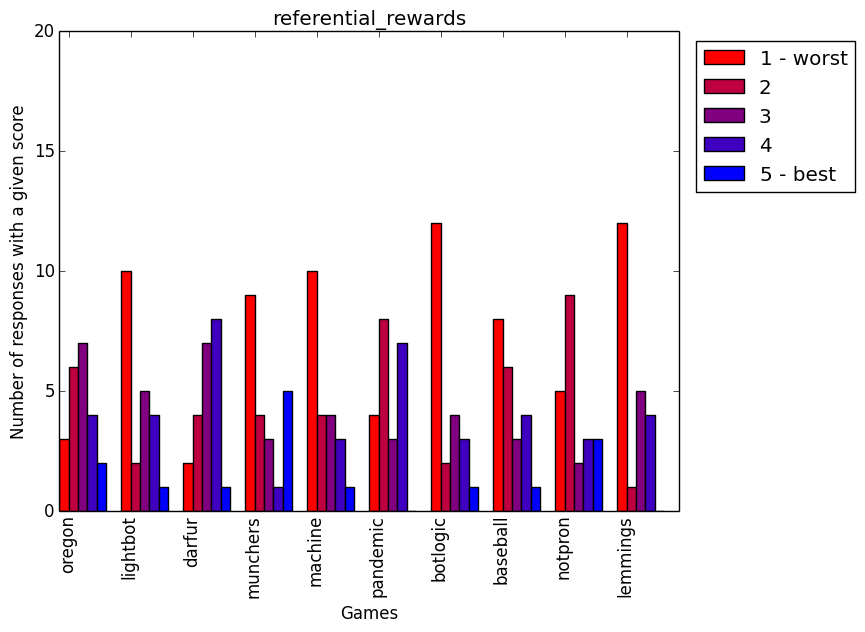
\includegraphics[width=\textwidth, height=.4\textheight, keepaspectratio=true]{referential_rewards_scores.png} 
				\caption{Rewards for knowing referential material}
				\end{figure}

				\textit{Darfur is Dying} was the only game with a significant positive score for referential rewards. This is expected, as the game contains situations where awareness of the conflict in Darfur directly affects gameplay (e.g. children should fetch the water instead of adults).

			\subsection{Reset time penalty for failure}
				\begin{figure}[] 
				\centering 
				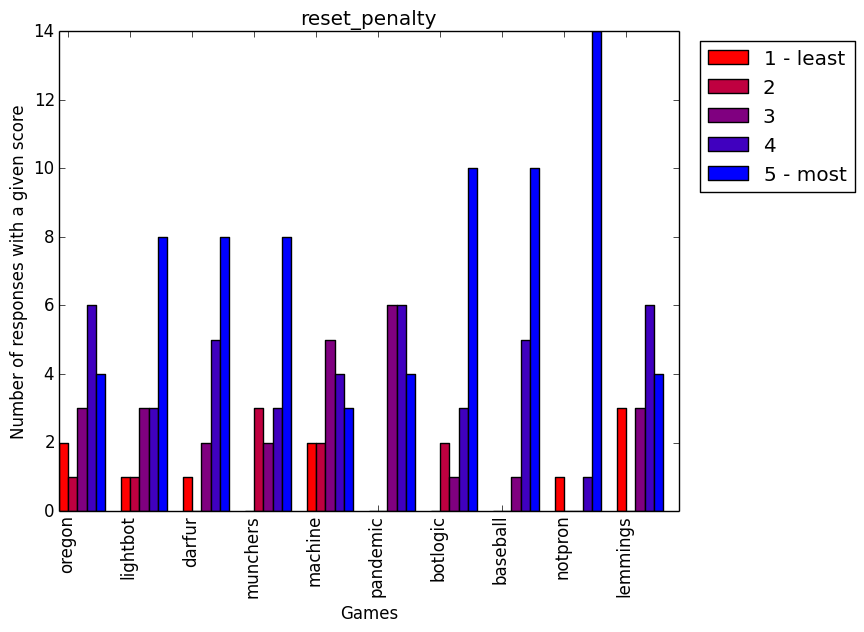
\includegraphics[width=\textwidth, height=.4\textheight, keepaspectratio=true]{reset_penalty_scores.png} 
				\caption{Reset time penalty for failure}
				\end{figure}

				In contrast to most of the other rubric items, the reset time penalty for failure recieved universally postitive scores for all games. This means that all the games were very effective about using the player's failure time wisely, or that the prompt or choices biased players towards positive responses.

			\subsection{Game resource penalty for failure}
				\begin{figure}[] 
				\centering 
				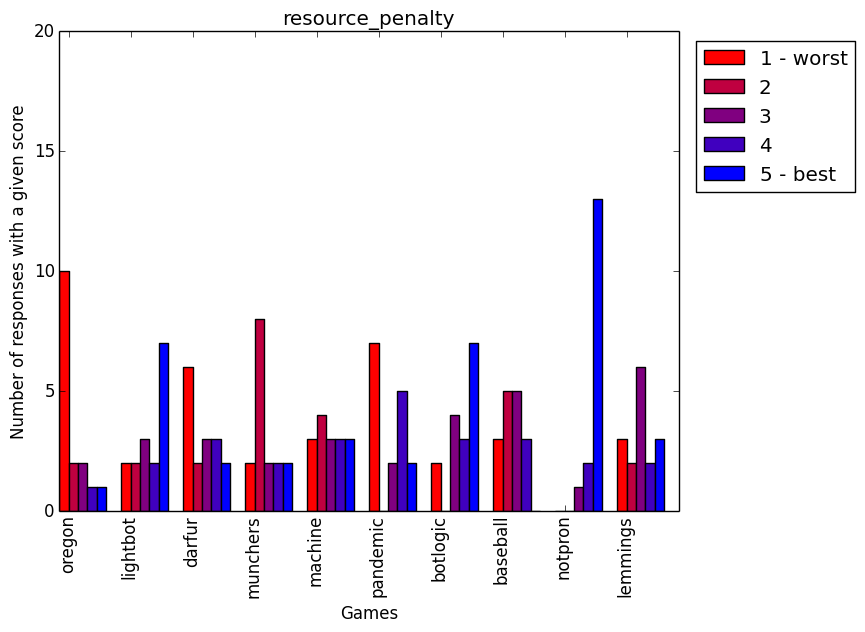
\includegraphics[width=\textwidth, height=.4\textheight, keepaspectratio=true]{resource_penalty_scores.png} 
				\caption{Game resource penalty for failure}
				\end{figure}

				The resource penalty for failure received some strong positive and negative ratings for games. \textit{The Oregon Trail, Number Munchers, and Pandemic} received negative ratings, which is somewhat expected; in the games, if the player fails, they usually have to restart the game. However, for \textit{Light Bot, Botlogic, and Notpron}, players can restart a failed level or puzzle immediately, usually with no penalty.

				It's important to note that raters may have confused game resource penalty with reset time penalty. It warrants further investigation, either into the survey prompts and choices, or into the games themselves.

			\clearpage

		\section{Game Scores}
			This section contains the scoring results for each game. For each game, a bar graph is given for each rubric item. These graphs are shown in Figures 6.30 through 6.39. Each bar graph contains the scores that the rubric item recieved for that game.

			An alternate visualization of this data, where each rubric item has a bar graph for all of the game, can be found in the previous section.

			\subsection{Math Baseball}

				\begin{figure}[] 
				\centering 
				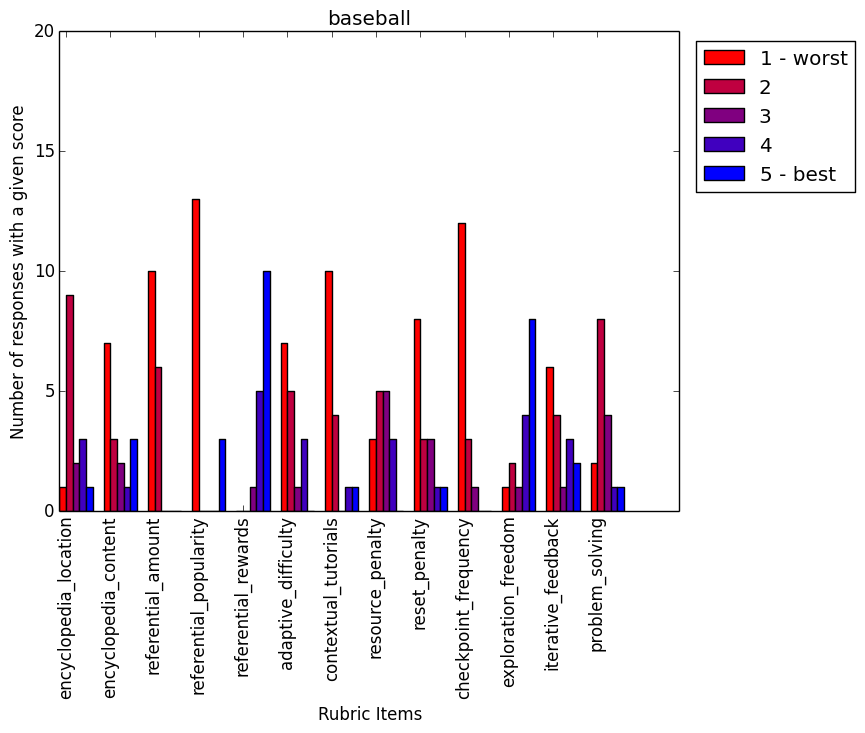
\includegraphics[width=\textwidth, height=.4\textheight, keepaspectratio=true]{baseball_scores.png} 
				\caption{Math Baseball}
				\end{figure}

				\textit{Math Baseball} scored well on the Popularity of Referential Material and the Reset time penalty. Popularity of Referential Material is easily explained, due to the prevalence of simple arithmetic in everyday life. The reset time penalty for \textit{Math Baseball} is also minimal; it takes seconds to set up a new game.

			\subsection{BotLogic}

				\begin{figure}[] 
				\centering 
				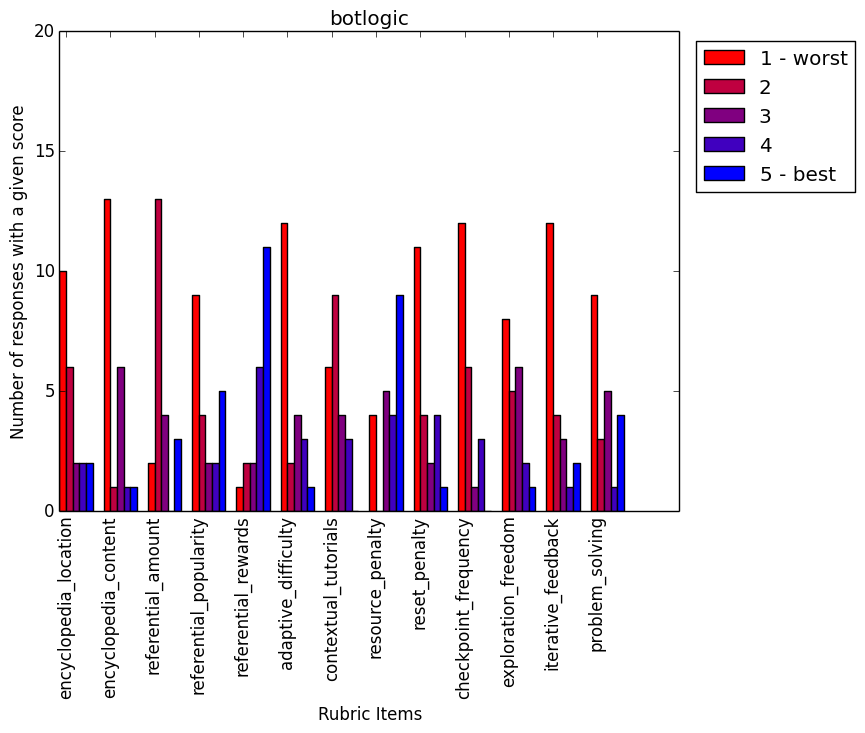
\includegraphics[width=\textwidth, height=.4\textheight, keepaspectratio=true]{botlogic_scores.png} 
				\caption{Botlogic}
				\end{figure}

				\textit{BotLogic} scored well on both the Game resource penalty and the Reset time penalty. In the game, if the player has a poorly written program, they only need to press the reset button to start the level over again, keeping all of their previous work. The high scores for both items are expected.

			\subsection{Darfur is Dying}

				\begin{figure}[] 
				\centering 
				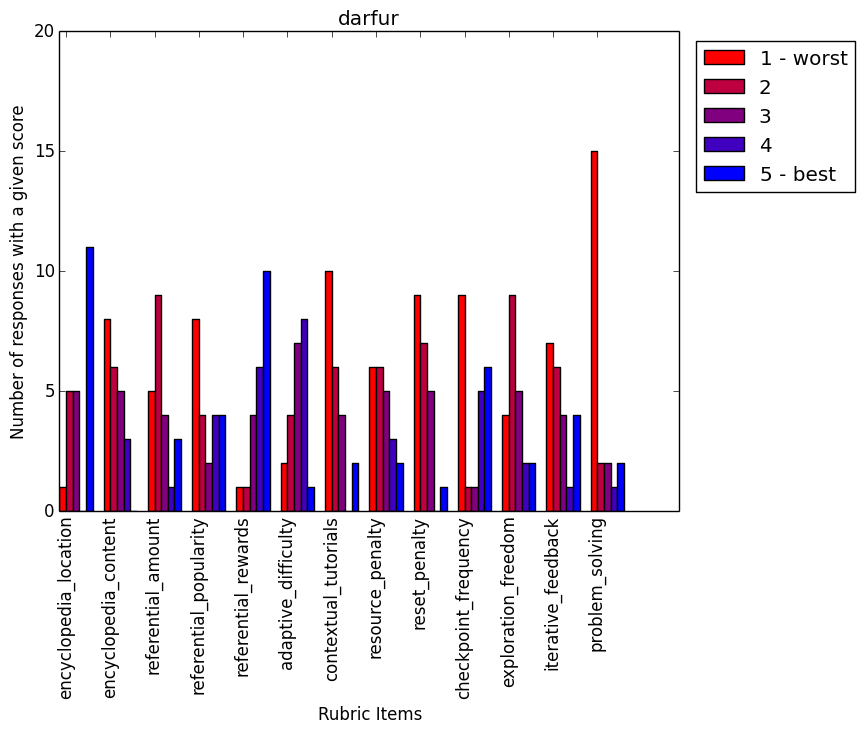
\includegraphics[width=\textwidth, height=.4\textheight, keepaspectratio=true]{darfur_scores.png} 
				\caption{Darfur is Dying}
				\end{figure}

				\textit{Darfur is Dying} scored well in the Amount of Referential Material, which is expected due to its purpose of advocacy. It also scores well on Reset Time Penalty; if players fail in the game, they're immediately taken back to a selection screen where they can start the challenge again.

			\subsection{Lemmings}

				\begin{figure}[] 
				\centering 
				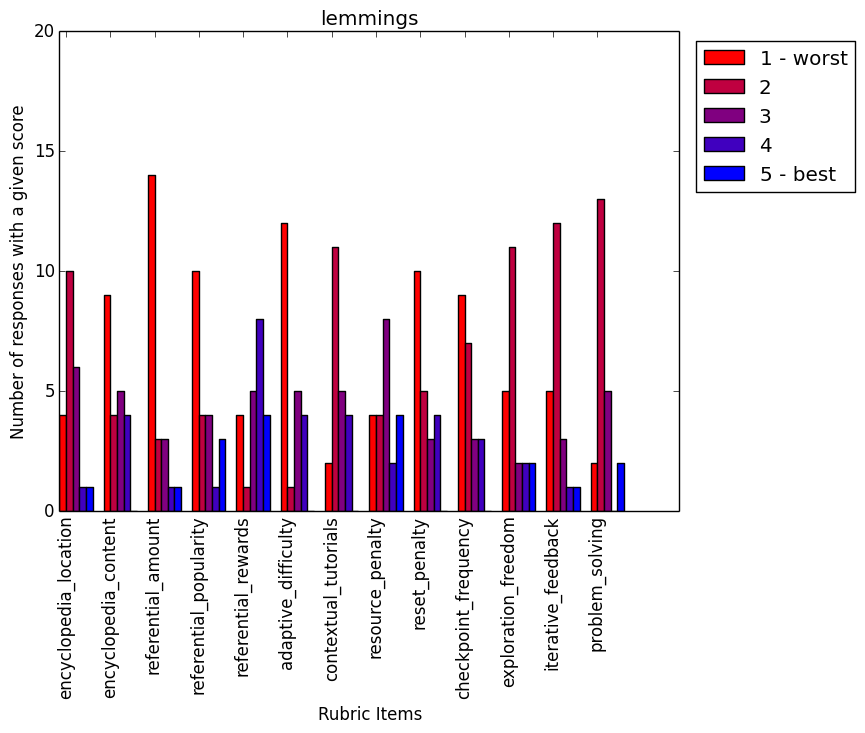
\includegraphics[width=\textwidth, height=.4\textheight, keepaspectratio=true]{lemmings_scores.png} 
				\caption{Lemmings}
				\end{figure}

				\textit{Lemmings} didn't score well in any items except marginally in Game Reset Penalty. This is expected, as level selection doesn't take very long.

			\subsection{Light Bot}

				\begin{figure}[] 
				\centering 
				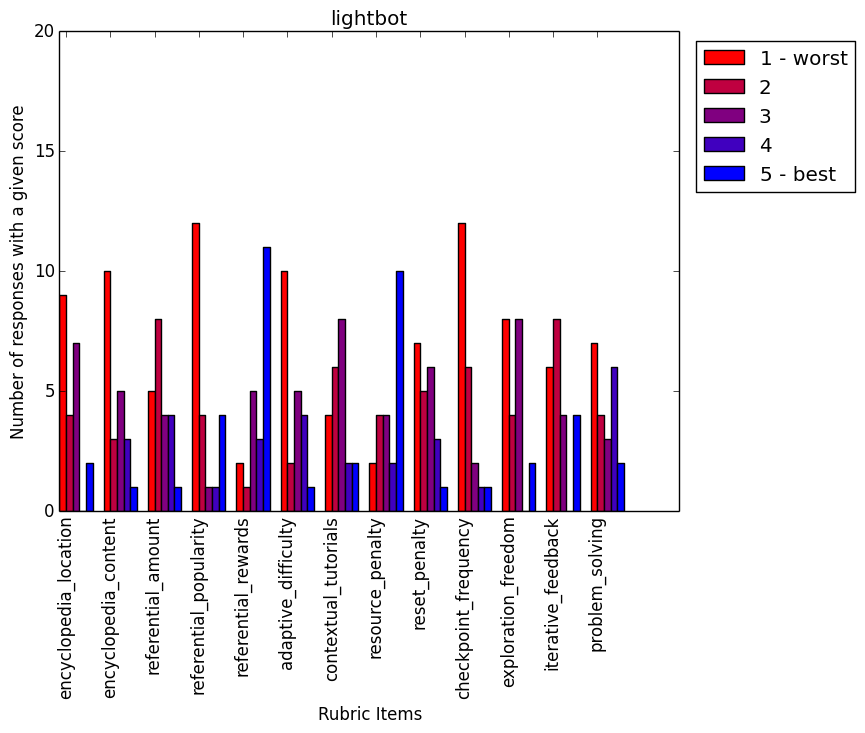
\includegraphics[width=\textwidth, height=.4\textheight, keepaspectratio=true]{lightbot_scores.png} 
				\caption{Light Bot}
				\end{figure}

				\textit{Light Bot} scored well on Game Resource Penalty and Reset Time Penalty. When a player has a faulty program, they can reset the level easily, keeping all of their existing work.

			\subsection{The Incredible Machine}

				\begin{figure}[] 
				\centering 
				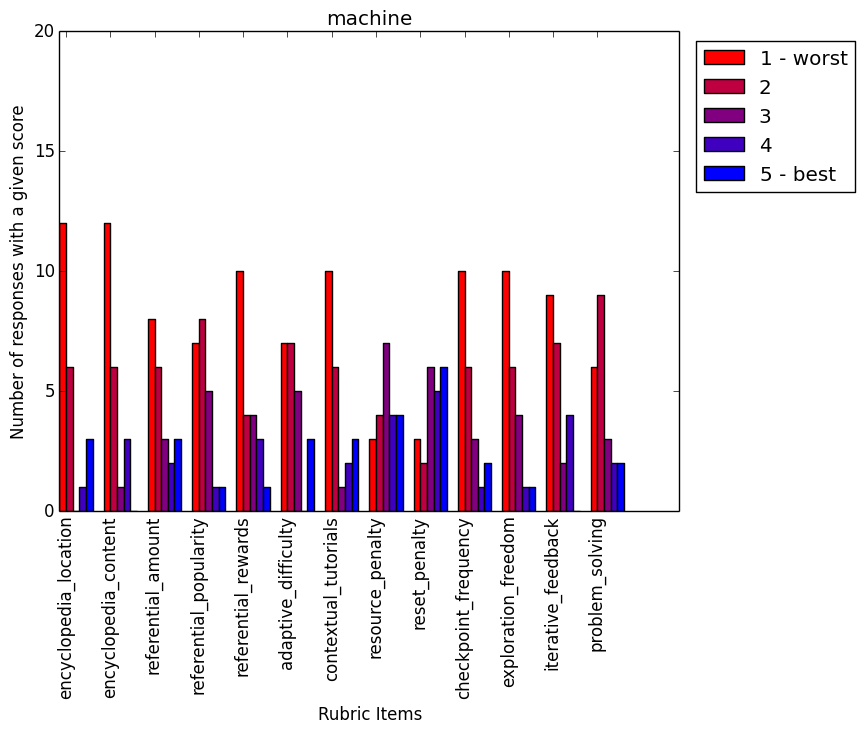
\includegraphics[width=\textwidth, height=.4\textheight, keepaspectratio=true]{machine_scores.png} 
				\caption{The Incredible Machine}
				\end{figure}

				\textit{The Incredible Machine} did not score exceptionally well on any rubric items.

			\subsection{Number Munchers}

				\begin{figure}[] 
				\centering 
				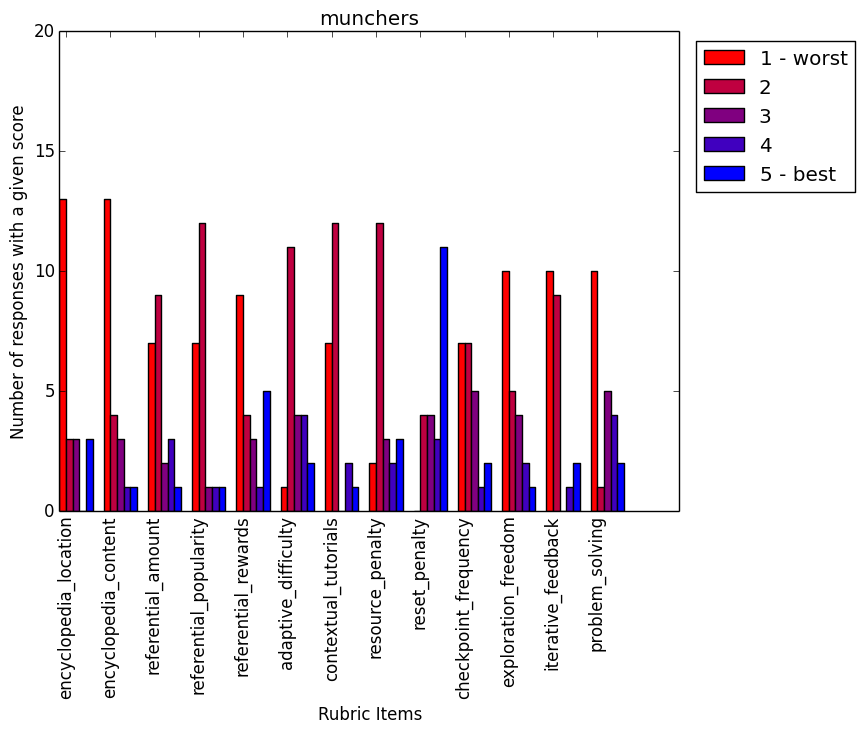
\includegraphics[width=\textwidth, height=.4\textheight, keepaspectratio=true]{munchers_scores.png} 
				\caption{Number Munchers}
				\end{figure}

				\textit{Number Munchers} only scored well in the Reset Time Penalty, which is expected for a level selection screen.

			\subsection{Notpron}

				\begin{figure}[] 
				\centering 
				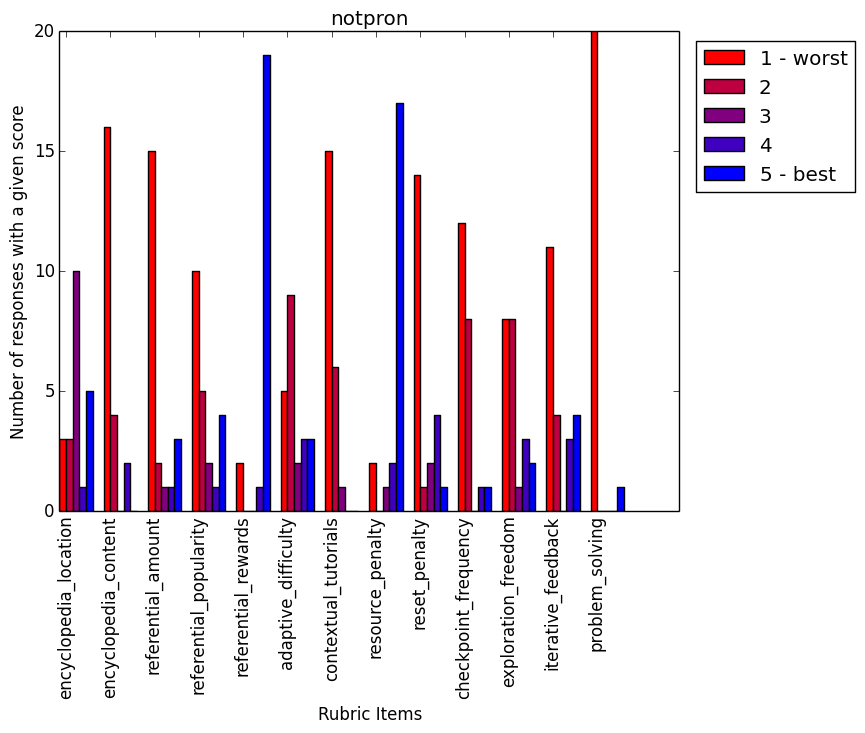
\includegraphics[width=\textwidth, height=.4\textheight, keepaspectratio=true]{notpron_scores.png} 
				\caption{Notpron}
				\end{figure}

				\textit{Notpron} scored very well in both the Game Resource Penalty and the Reset Time Penalty. Failing a challenge means that a player cannot continue until they've completed the challenge, and they keep all existing work and level progress.

			\subsection{The Oregon Trail}

				\begin{figure}[] 
				\centering 
				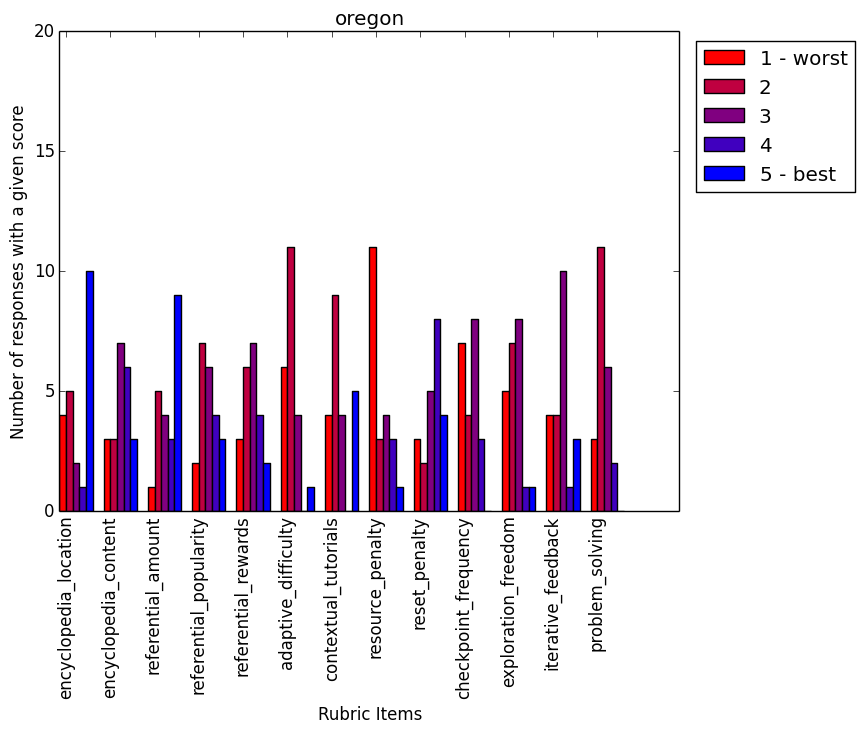
\includegraphics[width=\textwidth, height=.4\textheight, keepaspectratio=true]{oregon_scores.png} 
				\caption{The Oregon Trail}
				\end{figure}

				\textit{The Oregon Trail} scored highly on the Amount of Referential Information in the game, as well as the Location of the Game Encyclopedia. At the beginning of the game, players are taken through a large amount of historical and factual information about the Oregon Trail and pioneer life, so this result is expected.

			\subsection{Pandemic 2}

				\begin{figure}[] 
				\centering 
				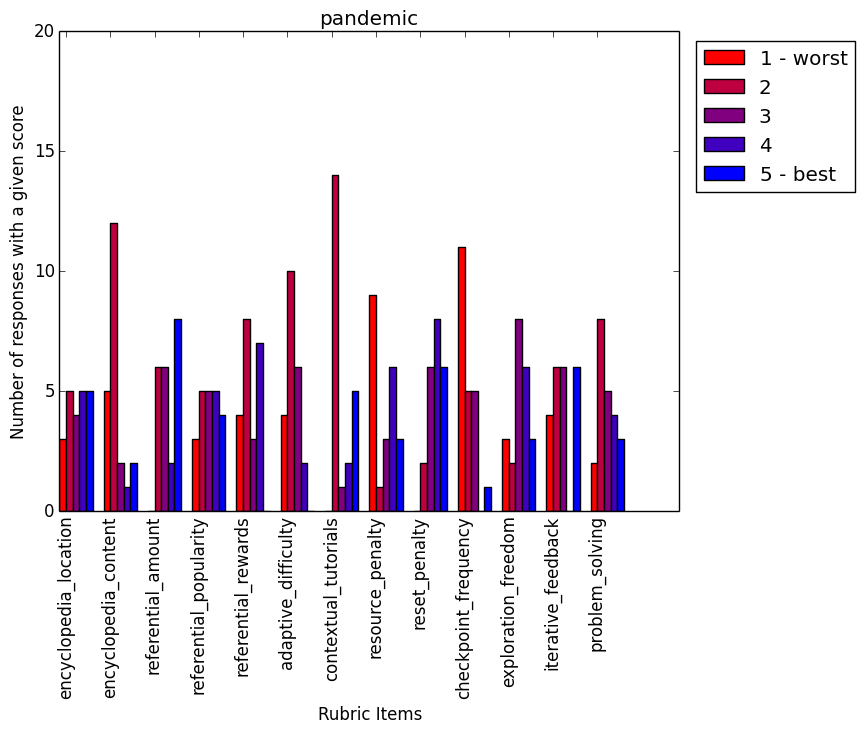
\includegraphics[width=\textwidth, height=.4\textheight, keepaspectratio=true]{pandemic_scores.png} 
				\caption{Pandemic 2}
				\end{figure}

				\textit{Pandemic 2} had very mixed views for most of the rubric items. This could indicate that the nature of education within the game is something that we haven't thought of yet, or that the rubric was inaccurate at addressing these items.

			\clearpage

		\section{Opinions on the fun and educational value of each game}

			At the end of the rubric section of the survey, players are asked four opinion questions; if the game was fun, if it was educational, if they had fun playing it, and if they learned anything while playing it. The responses were in Likert scale format.

			\subsection{Math Baseball}

				\begin{figure}[] 
				\centering 
				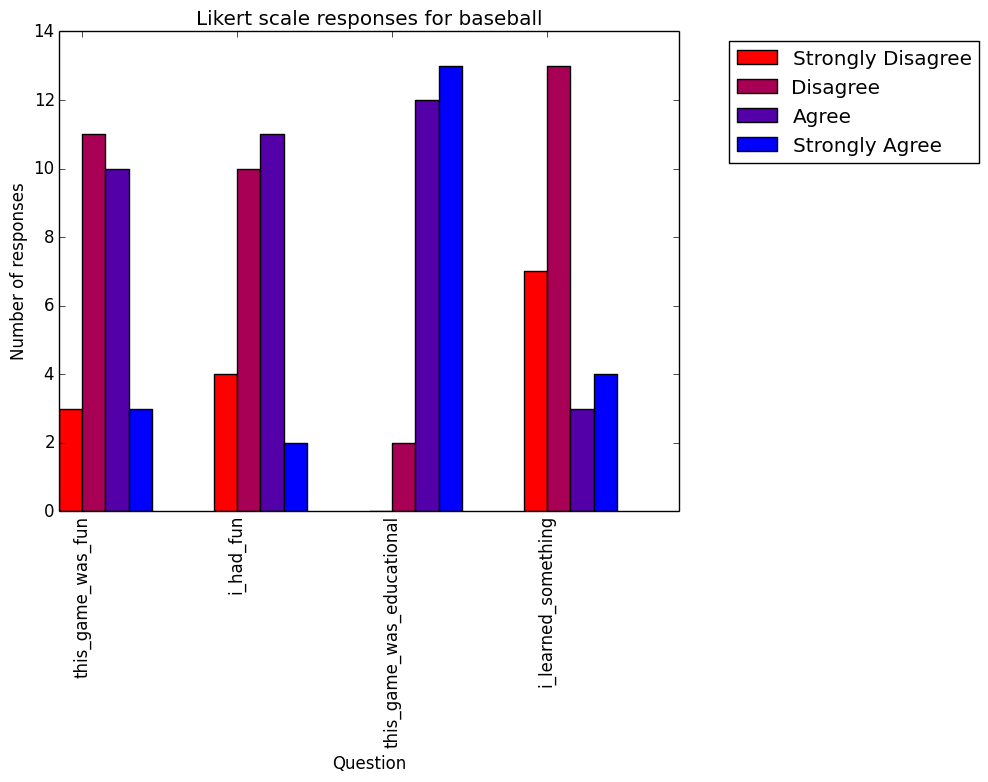
\includegraphics[width=\textwidth, height=.4\textheight, keepaspectratio=true]{baseball_likert.png} 
				\caption{Math Baseball}
				\end{figure}

				Players disagreed on whether or not \textit{Math Baseball} was fun, but agreed that it was definitely considered an educational game. However, most players didn't learn anything from this game, presumably due to the low grade level. It's also important to consider that the game doesn't teach anything new; it is designed to test students on material they are already familiar with.

			\subsection{Botlogic}

				\begin{figure}[] 
				\centering 
				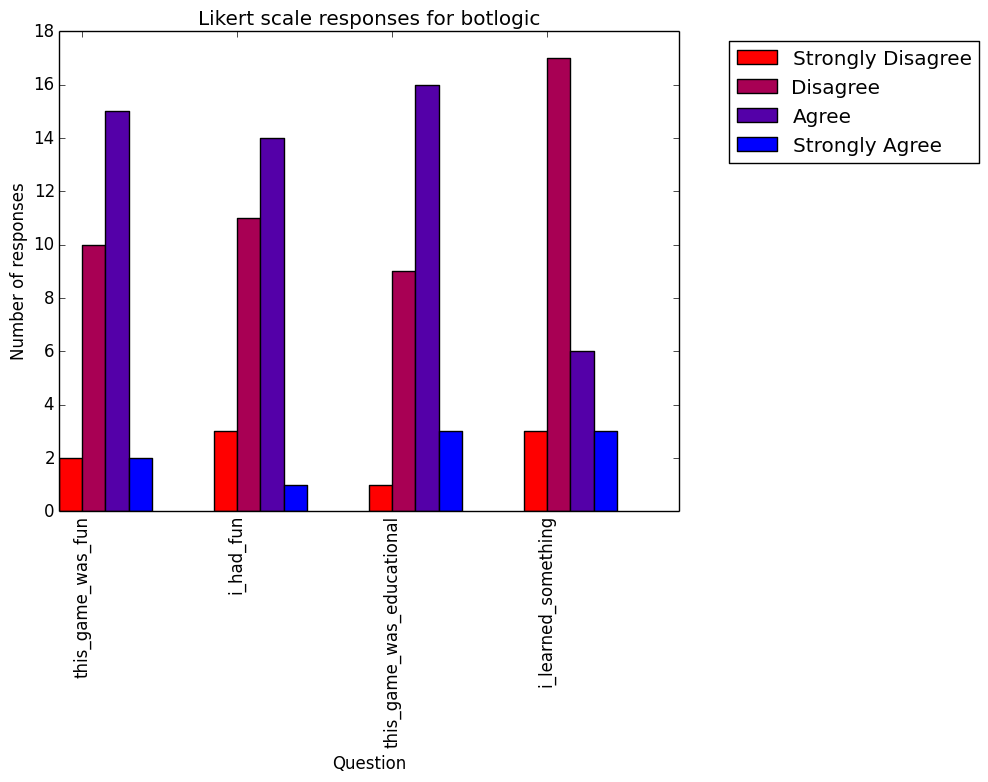
\includegraphics[width=\textwidth, height=.4\textheight, keepaspectratio=true]{botlogic_likert.png} 
				\caption{Botlogic}
				\end{figure}

				Players were largely ambivalent about the fun or educational content of \textit{Botlogic}, but did not learn much from the game. This could be due to the low grade level the game aims to teach content at. 

			\subsection{Darfur is Dying}

				\begin{figure}[] 
				\centering 
				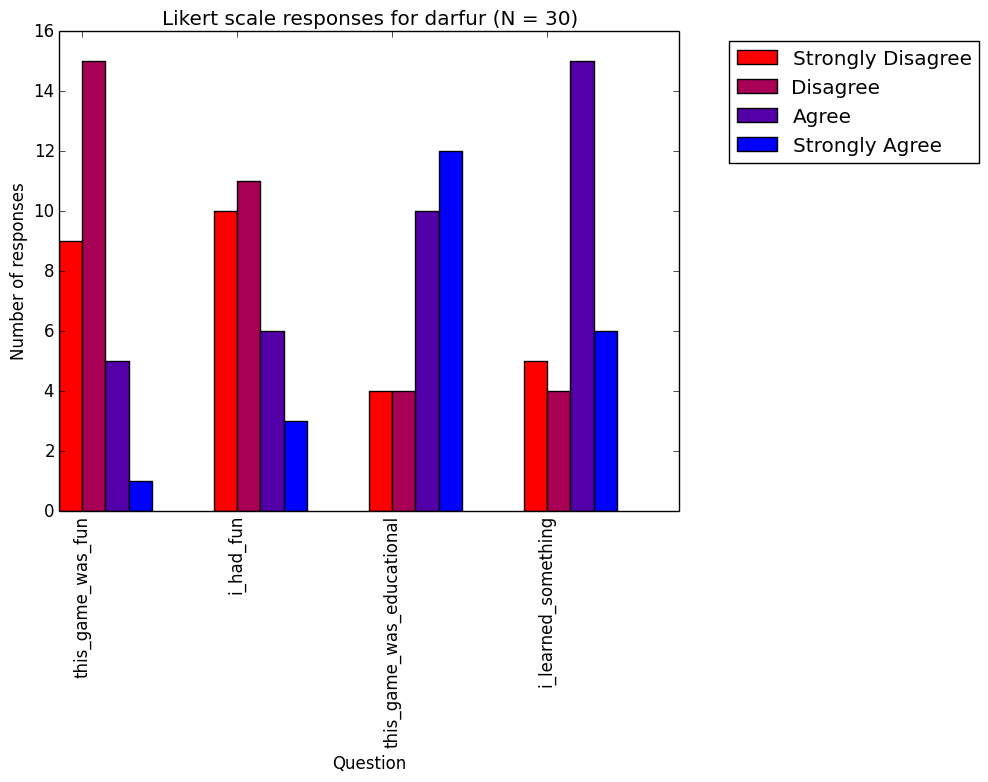
\includegraphics[width=\textwidth, height=.4\textheight, keepaspectratio=true]{darfur_likert.png} 
				\caption{Darfur is Dying}
				\end{figure}

				Players agreed that \textit{Darfur is Dying} was not a fun game, but it was an educational one, and one that they learned something from. It was effective at being educational, but likely not something players would willingly play.

			\subsection{Lemmings}

				\begin{figure}[] 
				\centering 
				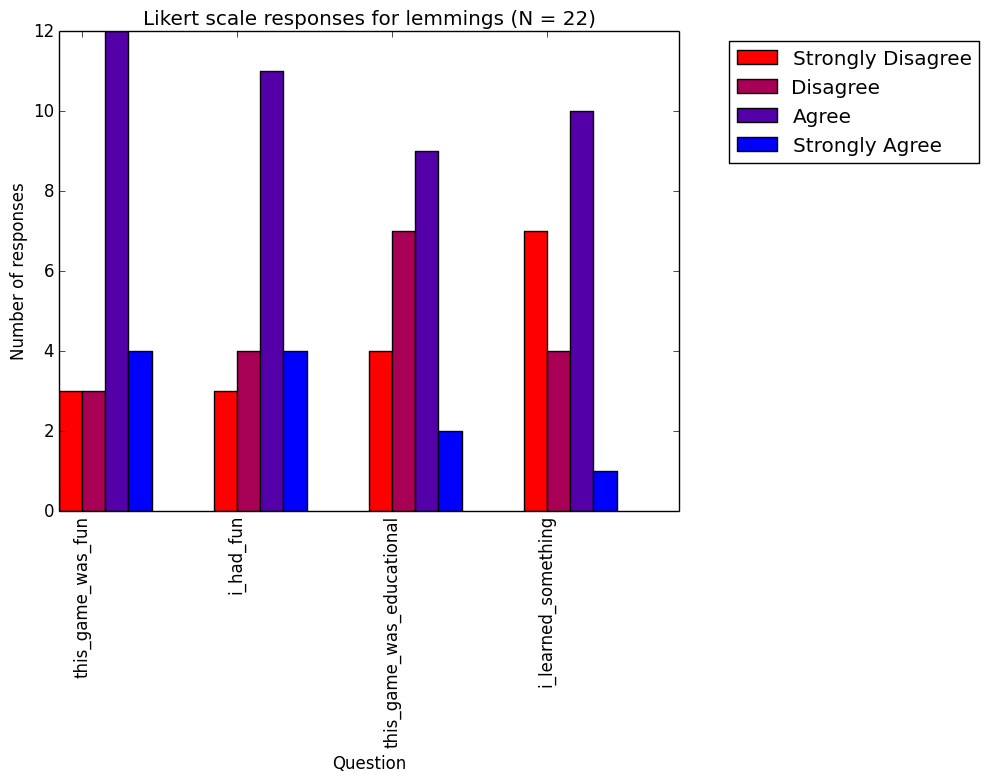
\includegraphics[width=\textwidth, height=.4\textheight, keepaspectratio=true]{lemmings_likert.png} 
				\caption{Lemmings}
				\end{figure}

				Players agreed that \textit{Lemmings} was fun, but had less agreement on the educational content of the game. As a primarily non-educational game, this is expected.

			\subsection{Light Bot}

				\begin{figure}[] 
				\centering 
				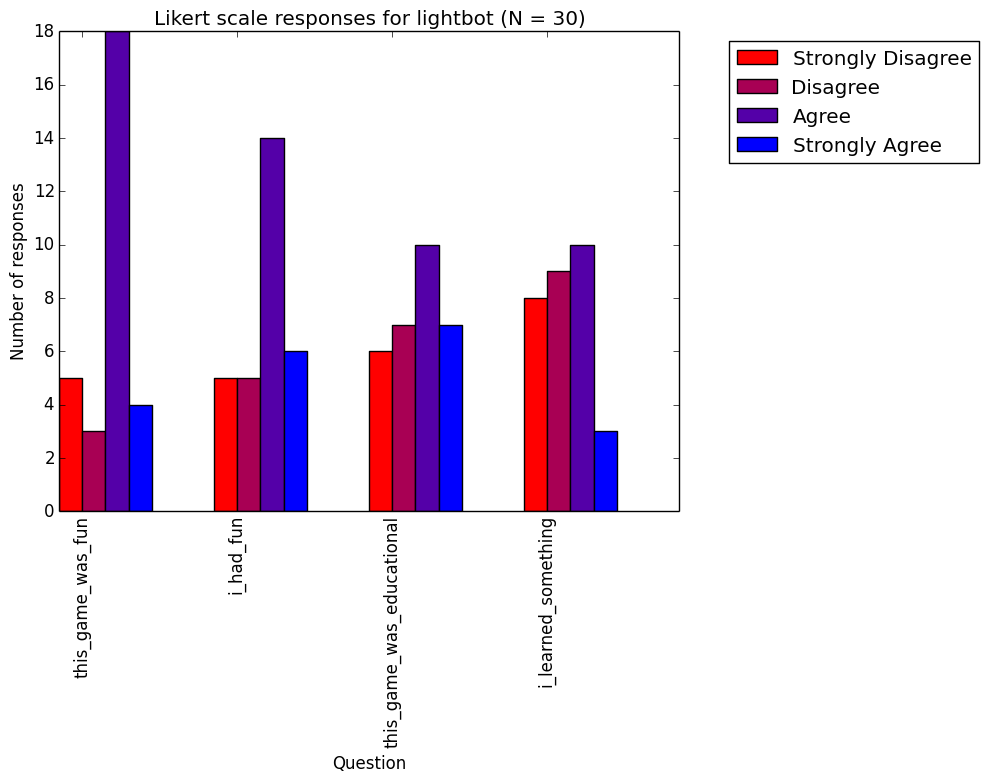
\includegraphics[width=\textwidth, height=.4\textheight, keepaspectratio=true]{lightbot_likert.png} 
				\caption{Light Bot}
				\end{figure}

				Players agreed that \textit{Light Bot} was fun, and that they had fun playing it, but were very conflicted on whether or not it was an educational game. 

				This is unusual, because \textit{Light Bot} was considered one of the more educational games selected. It's possible that most players didn't reach the `educational' part of \textit{Light Bot} (e.g. the functions and loops sections) due to their short play time.

			\subsection{The Incredible Machine}

				\begin{figure}[] 
				\centering 
				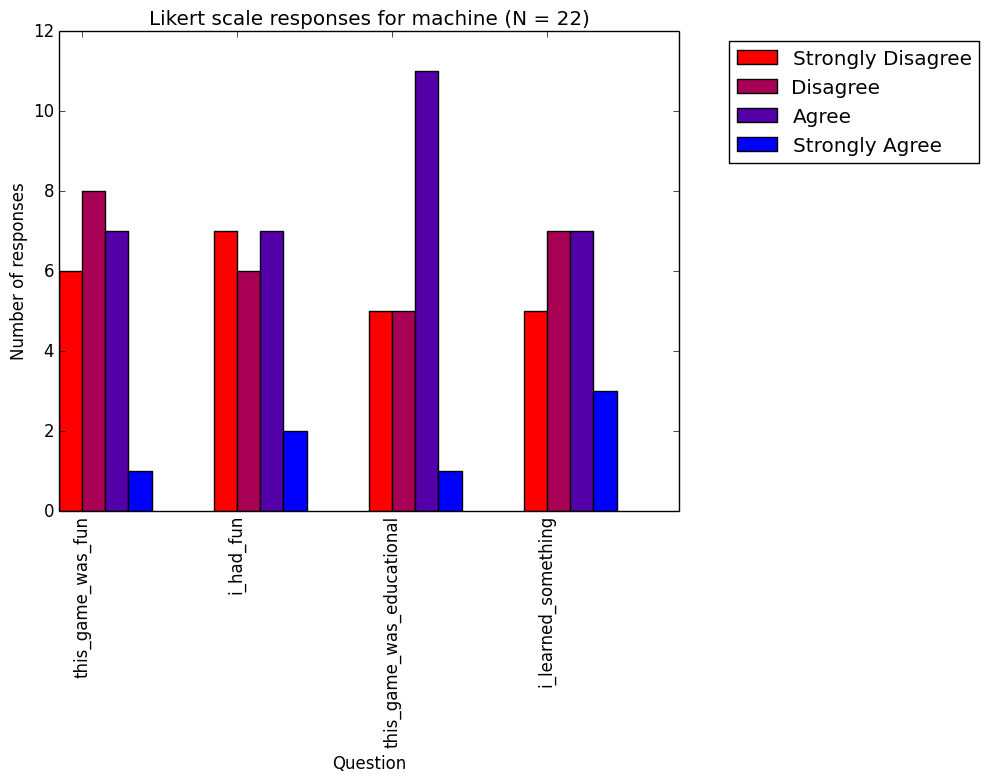
\includegraphics[width=\textwidth, height=.4\textheight, keepaspectratio=true]{machine_likert.png} 
				\caption{The Incredible Machine}
				\end{figure}

				Players were ambivalent about \textit{The Incredible Machine} being fun, as well as whether they had fun or learned anything while playing it. However, they did largely agree that it is an educational game.

			\subsection{Number Munchers}

				\begin{figure}[] 
				\centering 
				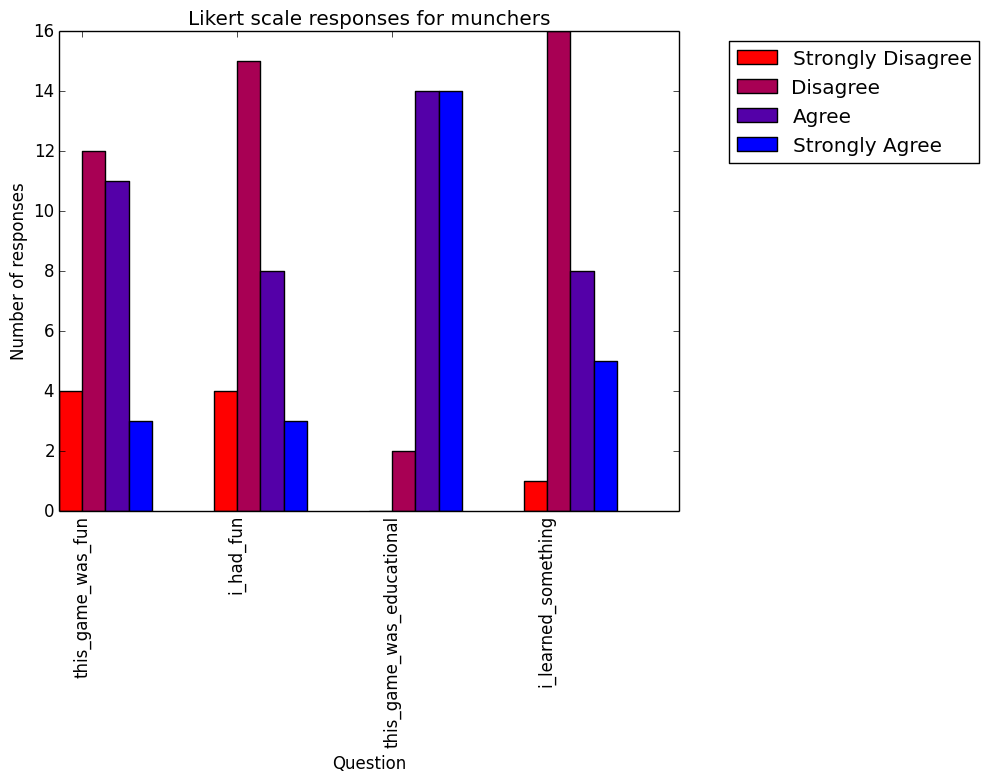
\includegraphics[width=\textwidth, height=.4\textheight, keepaspectratio=true]{munchers_likert.png} 
				\caption{Number Munchers}
				\end{figure}

				Players didn't have fun and didn't learn anything in \textit{Number Munchers}, but they agreed that it is an educational game. \textit{Number Munchers} teaches grade level math, so low scores on learning is expected.

			\subsection{Notpron}

				\begin{figure}[] 
				\centering 
				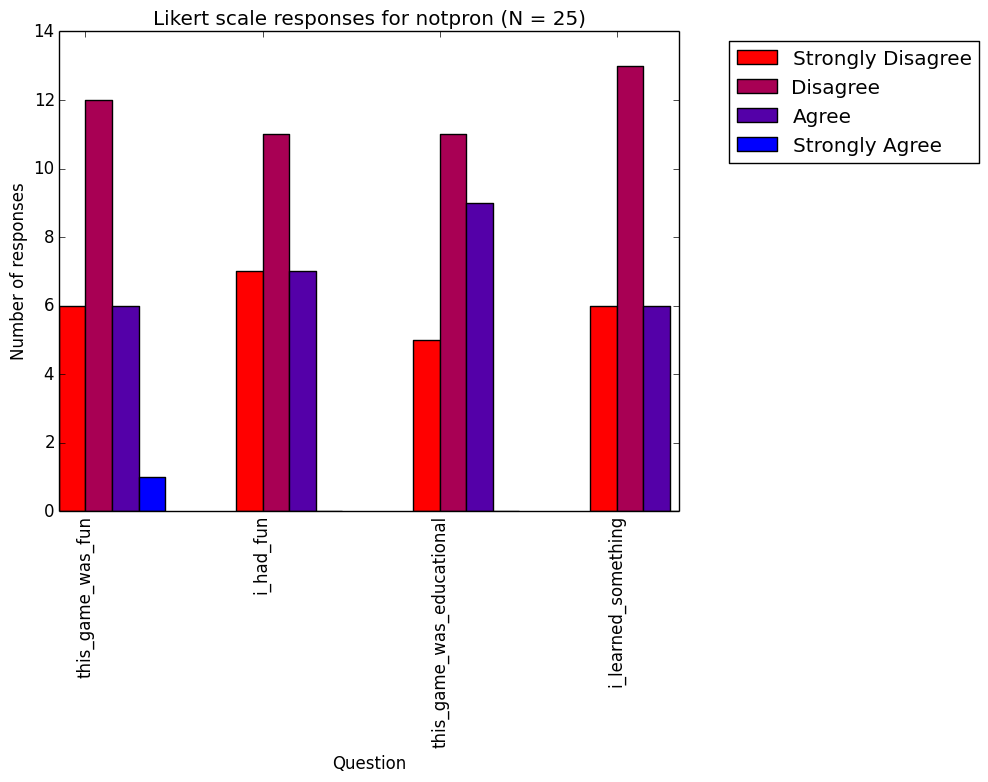
\includegraphics[width=\textwidth, height=.4\textheight, keepaspectratio=true]{notpron_likert.png} 
				\caption{Notpron}
				\end{figure}

				Players didn't have fun or learn anything in \textit{Notpron}, and didn't consider it a fun game. However, they were somewhat conflicted as to whether or not it was educational.

			\subsection{The Oregon Trail}

				\begin{figure}[] 
				\centering 
				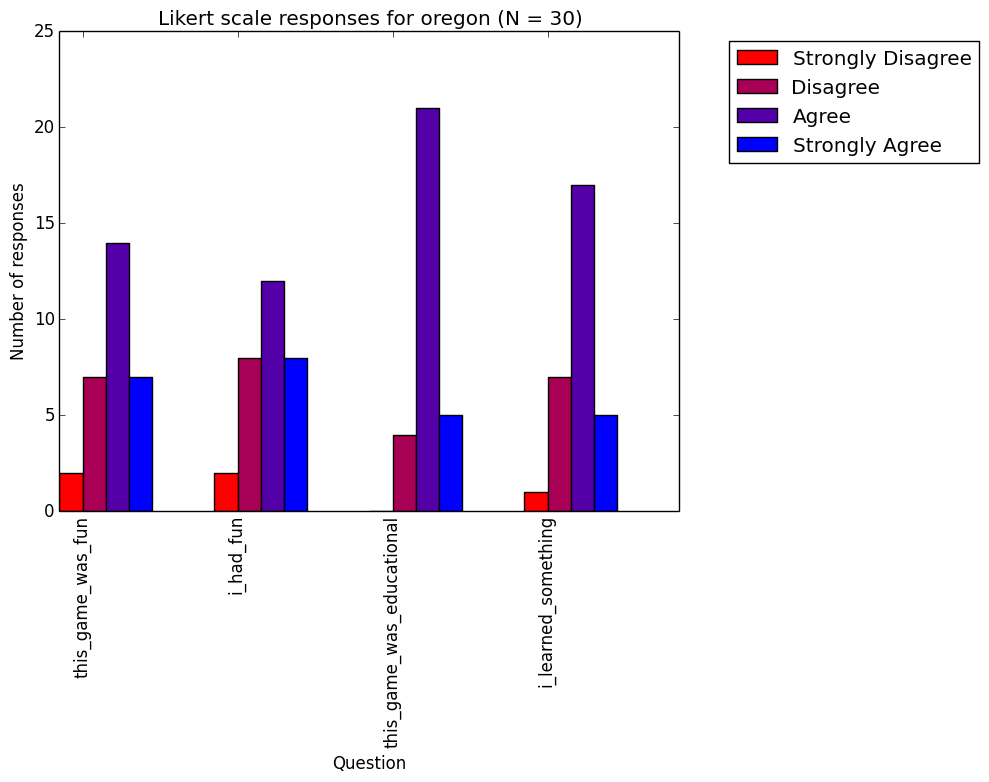
\includegraphics[width=\textwidth, height=.4\textheight, keepaspectratio=true]{oregon_likert.png} 
				\caption{The Oregon Trail}
				\end{figure}

				Players generally liked \textit{The Oregon Trail}; they had fun playing it, and learned something while doing so.

			\subsection{Pandemic 2}

				\begin{figure}[] 
				\centering 
				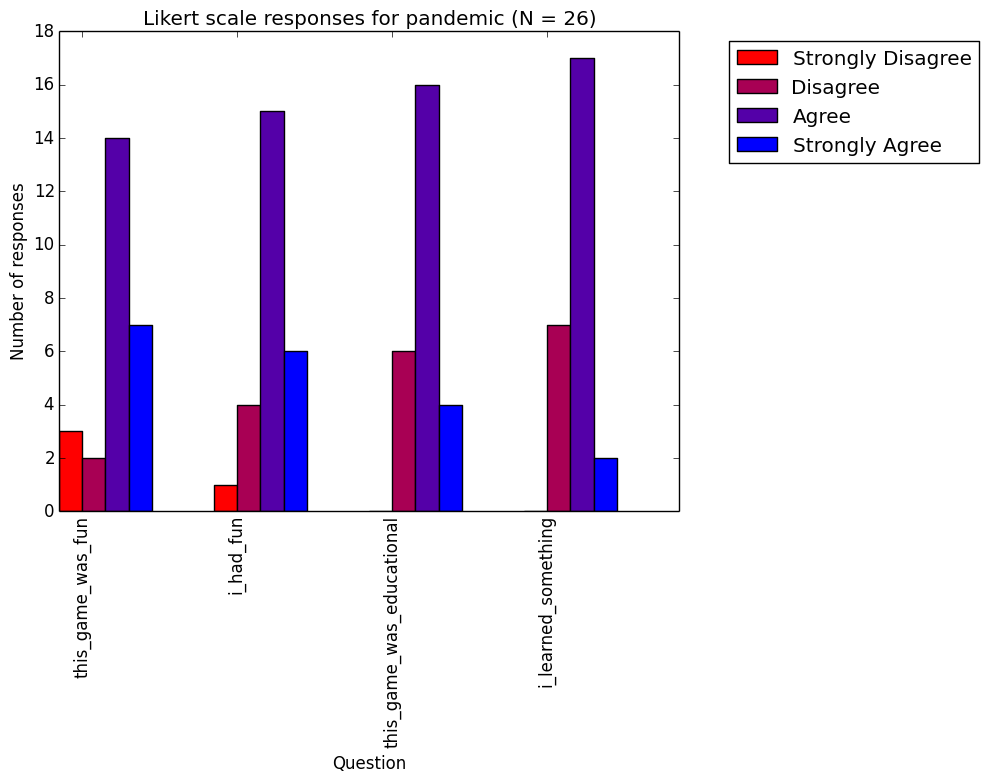
\includegraphics[width=\textwidth, height=.4\textheight, keepaspectratio=true]{pandemic_likert.png} 
				\caption{Pandemic 2}
				\end{figure}

				This was one of the more unexpected results was with Pandemic 2. Across the board, players lightly agreed that \textit{Pandemic 2} was a fun and educational game, and that they both had fun and learned something while playing it. The fun responses to the game were expected, but the educational ones were not; the game was selected due to its potential for tangential learning.

			\clearpage

